\documentclass[sn-mathphys-num,a4paper,iicol,lineno,pdflatex]{sn-jnl-hacked}
%%% RB: Hacking style to resemble camera ready layout of main text

% !TEX root =  ./main.tex


%%% RB additional packages
\usepackage[english]{babel}
\usepackage[T1]{fontenc}
\usepackage{listings}
\usepackage{comment}
\usepackage[normalem]{ulem}
\usepackage{hyphenat}
\usepackage{stmaryrd}
%\usepackage{wasysym}
\usepackage{proof} 
\usepackage{bussproofs}
 \usepackage[all]{xy}
\usepackage{mathtools} 
%\usepackage{lscape}
%\usepackage{cancel}
\usepackage{xspace}
\usepackage{subcaption}
\usepackage[textsize=tiny]{todonotes}
% Load hyperref (and then cleveref) last
\usepackage{hyperref}
\usepackage{cleveref}

\captionsetup[subfigure]{justification=centering}

%\usepackage[inline]{enumitem}
\newcommand{\lab}[1]{\textsf{#1}}
\newcommand{\blab}[1]{\lab{\bfseries #1}}
\newcommand{\ilab}[1]{\lab{\itshape #1}}

\newcommand{\nil}{\mathbf{0}}
\newcommand{\obs}[2]{\langle #1\vartriangleright #2\rangle}
\newcommand{\ccoin}{{\text{\sffamily ccoin}}\xspace}
\newcommand{\tcoin}{{\text{\sffamily tcoin}}\xspace}
\newcommand{\cpowder}{{\text{\sffamily cpowder}}\xspace}
\newcommand{\tpowder}{{\text{\sffamily tpowder}}\xspace}
\newcommand{\nomilk}{{\text{\sffamily nomilk}}\xspace}
\newcommand{\cappuccino}{{\text{\sffamily cappuccino}}\xspace}
\newcommand{\espresso}{{\text{\sffamily espresso}}\xspace}
\newcommand{\tea}{{\text{\sffamily tea}}\xspace}
\newcommand{\idle}{{\text{\sffamily idle}}\xspace}
\newcommand{\am}{{\text{\sffamily am}}\xspace}
\newcommand{\anger}{{\text{\sffamily anger}}\xspace}
\newcommand{\bang}{{\text{\sffamily bang}}\xspace}
\newcommand{\Forbidden}{{\text{\sffamily Forbidden}}\xspace}

\newcommand{\BioResolve}{\textsf{BioResolve}\xspace}
\newcommand{\GROOVE}{\textsf{GROOVE}\xspace}

% Node types
\newcommand{\Reaction}{{\text{\bfseries\sffamily Reaction}}\xspace}
\newcommand{\Rule}{{\text{\bfseries\sffamily Rule}}\xspace}
\newcommand{\Step}{{\text{\bfseries\sffamily Step}}\xspace}
\newcommand{\Entity}{{\text{\bfseries\sffamily Entity}}\xspace}
\newcommand{\State}{{\text{\bfseries\sffamily State}}\xspace}
\newcommand{\Token}{{\text{\bfseries\sffamily Token}}\xspace}
\newcommand{\RuleOcc}{{\text{\bfseries\sffamily RuleOcc}}\xspace}
\newcommand{\EntityInst}{{\text{\bfseries\sffamily EntityInst}}\xspace}
% Edges
\newcommand{\inhibitor}{{\text{\sffamily inhibitor}}\xspace}
\newcommand{\product}{{\text{\sffamily product}}\xspace}
\newcommand{\reactant}{{\text{\sffamily reactant}}\xspace}
\newcommand{\nextt}{{\text{\sffamily next}}\xspace}
\newcommand{\move}{{\text{\sffamily move}}\xspace}
% Flags
\newcommand{\fired}{{\text{\sffamily\itshape fired}}\xspace}
\newcommand{\present}{{\text{\sffamily\itshape present}}\xspace}
% Rules
\newcommand{\contextR}{{\text{\sffamily context}}\xspace}
\newcommand{\reactR}{{\text{\sffamily react}}\xspace}
\newcommand{\firedR}{{\text{\sffamily fired}}\xspace}


%Version 3 October 2023
% See section 11 of the User Manual for version history
%
%%%%%%%%%%%%%%%%%%%%%%%%%%%%%%%%%%%%%%%%%%%%%%%%%%%%%%%%%%%%%%%%%%%%%%
%%                                                                 %%
%% Please do not use \input{...} to include other tex files.       %%
%% Submit your LaTeX manuscript as one .tex document.              %%
%%                                                                 %%
%% All additional figures and files should be attached             %%
%% separately and not embedded in the \TeX\ document itself.       %%
%%                                                                 %%
%%%%%%%%%%%%%%%%%%%%%%%%%%%%%%%%%%%%%%%%%%%%%%%%%%%%%%%%%%%%%%%%%%%%%

%%\documentclass[referee,sn-basic]{sn-jnl}% referee option is meant for double line spacing

%%=======================================================%%
%% to print line numbers in the margin use lineno option %%
%%=======================================================%%

%%\documentclass[lineno,sn-basic]{sn-jnl}% Basic Springer Nature Reference Style/Chemistry Reference Style

%%======================================================%%
%% to compile with pdflatex/xelatex use pdflatex option %%
%%======================================================%%

%%\documentclass[pdflatex,sn-basic]{sn-jnl}% Basic Springer Nature Reference Style/Chemistry Reference Style

%%Note: the following reference styles support Namedate and Numbered referencing. By default the style follows the most common style. To switch between the options you can add or remove “Numbered” in the optional parenthesis. 
%%The option is available for: sn-basic.bst, sn-vancouver.bst, sn-chicago.bst%  
 
%%\documentclass[sn-nature]{sn-jnl}% Style for submissions to Nature Portfolio journals
%%\documentclass[sn-basic]{sn-jnl}% Basic Springer Nature Reference Style/Chemistry Reference Style
%%\documentclass[sn-mathphys-num]{sn-jnl}% Math and Physical Sciences Numbered Reference Style 
%%\documentclass[sn-mathphys-ay]{sn-jnl}% Math and Physical Sciences Author Year Reference Style
%%\documentclass[sn-aps]{sn-jnl}% American Physical Society (APS) Reference Style
%%\documentclass[sn-vancouver,Numbered]{sn-jnl}% Vancouver Reference Style
%%\documentclass[sn-apa]{sn-jnl}% APA Reference Style 
%%\documentclass[sn-chicago]{sn-jnl}% Chicago-based Humanities Reference Style

%%%% Standard Packages
%%<additional latex packages if required can be included here>

\usepackage{graphicx}%
\usepackage{multirow}%
\usepackage{amsmath,amssymb,amsfonts}%
\usepackage{amsthm}%
\usepackage{mathrsfs}%
\usepackage[title]{appendix}%
\usepackage{xcolor}%
\usepackage{textcomp}%
\usepackage{manyfoot}%
\usepackage{booktabs}%
\usepackage{algorithm}%
\usepackage{algorithmicx}%
\usepackage{algpseudocode}%
\usepackage{listings}%
%%%%

%%%%%=============================================================================%%%%
%%%%  Remarks: This template is provided to aid authors with the preparation
%%%%  of original research articles intended for submission to journals published 
%%%%  by Springer Nature. The guidance has been prepared in partnership with 
%%%%  production teams to conform to Springer Nature technical requirements. 
%%%%  Editorial and presentation requirements differ among journal portfolios and 
%%%%  research disciplines. You may find sections in this template are irrelevant 
%%%%  to your work and are empowered to omit any such section if allowed by the 
%%%%  journal you intend to submit to. The submission guidelines and policies 
%%%%  of the journal take precedence. A detailed User Manual is available in the 
%%%%  template package for technical guidance.
%%%%%=============================================================================%%%%

%%% as per the requirement new theorem styles can be included as shown below
%\theoremstyle{thmstyleone}%
%\newtheorem{theorem}{Theorem}%  meant for continuous numbers
%%%\newtheorem{theorem}{Theorem}[section]% meant for sectionwise numbers
%%% optional argument [theorem] produces theorem numbering sequence instead of independent numbers for Proposition
%\newtheorem{proposition}[theorem]{Proposition}% 
%%%\newtheorem{proposition}{Proposition}% to get separate numbers for theorem and proposition etc.
%
%\theoremstyle{thmstyletwo}%
%\newtheorem{example}{Example}%
%\newtheorem{remark}{Remark}%
%
%\theoremstyle{thmstylethree}%
%\newtheorem{definition}{Definition}%


\newtheoremstyle{thmwithspace}% Nome dello stile
  {5pt}% Spazio sopra
  {5pt}% Spazio sotto
  {\itshape}% Corpo del teorema
  {}% Indentazione
  {\bfseries}% Stile dell'intestazione
  {.}% Punteggiatura dopo l'intestazione
  { }% Spazio dopo l'intestazione
  {}% Specifica personalizzata per l'intestazione

%\theoremstyle{thmstyletwo}%
\theoremstyle{thmwithspace}%
\newtheorem{example}{Example}%
\newtheorem{remark}{Remark}%
%
%\theoremstyle{thmstylethree}%
\theoremstyle{thmwithspace}%
\newtheorem{definition}{Definition}%
\newtheorem{theorem}{Theorem}%
\newtheorem{lemma}[theorem]{Lemma}%
\newtheorem{proposition}[theorem]{Proposition}%
\newtheorem{corollary}[theorem]{Corollary}%

%\raggedbottom
%%\unnumbered% uncomment this for unnumbered level heads

%%%%%% To display ORCID Logo with link, Please add below definition and copy the ORCID_Color.eps in the manuscript package %%%%%
\makeatletter
	\def\@citecolor{blue}%
	\def\@urlcolor{blue}%
	\def\@linkcolor{blue}%
	\def\UrlFont{\rmfamily}
	\def\orcidID#1{\href{http://orcid.org/#1}{
\includegraphics{ORCID_Color.eps}}}
\makeatother

\begin{document}

\title[Experimenting with Reaction Systems using Graph Transformation]{Experimenting with Reaction Systems using Graph Transformation and GROOVE}

%%=============================================================%%
%% GivenName	-> \fnm{Joergen W.}
%% Particle	-> \spfx{van der} -> surname prefix
%% FamilyName	-> \sur{Ploeg}
%% Suffix	-> \sfx{IV}
%% \author*[1,2]{\fnm{Joergen W.} \spfx{van der} \sur{Ploeg} 
%%  \sfx{IV}}\email{iauthor@gmail.com}
%%=============================================================%%

\author[1]{\fnm{Roberto} \sur{Bruni\orcidID{0000-0002-7771-4154}}}\email{roberto.bruni@unipi.it}
%\equalcont{These authors contributed equally to this work.}

\author*[2]{\fnm{Arend} \sur{Rensink\orcidID{0000-0002-1714-6319}}}\email{arend.rensink@utwente.nl}
%\equalcont{These authors contributed equally to this work.}

\affil[1]{\orgdiv{CS Dept.}, \orgname{University of Pisa}, \orgaddress{\street{Largo B.\ Pontecorvo, 3}, \city{Pisa}, \postcode{56127},  \country{Italy}}}

\affil*[2]{\orgdiv{CS Dept.}, \orgname{University of Twente}, \orgaddress{\street{Hallenweg 19}, \city{Enschede}, \postcode{7522}, \country{Netherlands}}}

\abstract{We explore the capabilities of \GROOVE, a state-of-the-art toolset based on graph transformation systems, to perform reachability and causal analysis of Reaction Systems.
Our results are still preliminary, but encouraging, as in the presence of large state spaces \GROOVE outperforms available applications by halving the analysis time of both reachability and causal analyses.
From the point of view of \GROOVE, the implementation of Reaction Systems provided some interesting insights on the most convenient way to model certain computational requirements through negative and nested application conditions.}

\keywords{Reaction Systems, Graph Transformation, \GROOVE, \textcolor{red}{Other keywords}}

%%\pacs[JEL Classification]{D8, H51}

%%\pacs[MSC Classification]{35A01, 65L10, 65L12, 65L20, 65L70}

\maketitle

% !TEX root =  ./main.tex

\section{Introduction}

We explore the capabilities of a state-of-the-art toolset based on graph transformation to perform reachability, causal analysis and verification of complex systems modelled using Reaction Systems.

Reaction systems (RSs)~\cite{DBLP:journals/fuin/EhrenfeuchtR07} are a computational model inspired by the functioning of biochemical reactions within living cells. 
%The primary motivation behind RS is to provide a simple yet expressive model for understanding and analysing processes in natural and artificial systems.
RSs focus on the interaction of entities through a set of reactions. 
Each reaction relies on some reactants, inhibitors, and products to mimic two fundamental mechanisms found in nature: facilitation and inhibition.
%Facilitation means that a reaction can occur only if all of its reactants are present, while inhibition means that a reaction cannot occur if any of its inhibitors is present. 
At each time instant, the next state of the system is determined by the products of all enabled reactions plus some additional entities that are possibly provided by the environment.
Unlike traditional models of concurrency, like Petri nets, the theory of RSs is based on three principles: \emph{no permanency}: any entity vanishes unless it is sustained by a reaction; \emph{no competition}: an entity is either available for all reactions, or it is not available at all; and \emph{no counting}: the exact concentration level of available entities is ignored.
Moreover, due to the use of inhibitors, RS can exhibit non-monotonic behaviour, in the sense that what can be done with fewer resources is not necessarily replicable with more resources.

While \emph{closed} RSs evolve in isolation, \emph{interactive processes} are dealt with by providing suitable environments that provide a sequence of stimuli at each step: these are sets of entities that can be used to trigger or inhibit some reactions. A common example involves using contexts to analyse how drug administration affects organisms that are modelled as sets of reactions.

Since their introduction, RSs have been successfully applied to the analysis of complex systems in many different fields~\cite{ABP14,CMMBM12,Az17,OY16,DBLP:journals/ijfcs/EhrenfeuchtMR10,DBLP:journals/ijfcs/EhrenfeuchtMR11}.
Recent applications concerned, e.g., with the efficacy of medical treatments for comorbidities and with the selection of the best environment to achieve some desired phenomena~\cite{DBLP:conf/cmsb/BowlesBBFGM24,datamod2023}, led to experimenting with environments that exhibit nondeterministic and recursive behaviour.
As a consequence, performing reachability and causal analysis requires the exploration of large state spaces, for which the prototype tool \BioResolve~\cite{DBLP:journals/tcs/BrodoBF21} struggled in terms of  memory consumption and response time.
 
Graph Transformation (GT)~\cite{DBLP:series/eatcs/EhrigEPT06,DBLP:books/sp/HeckelT20} is a modelling technique that is widely applicable in problem domains where the objects of study have an inherent graphical structure, and the task at hand is to study their properties and evolution. Besides the graphs themselves, the core concept is that of a (transformation) \emph{rule} capturing a particular change to such a graph. Rules can be used, for instance, to describe the change of a system over time, but can also be instrumental in composing and decomposing graphs and so exposing structural properties.
Since RSs can be derived from Boolean network models and visualised themselves as suitable networks of reactions, it is quite natural trying to embed them within the GT framework to take advantage of well established analysis techniques.\footnote{\textcolor{blue}{It should be noted that there is another, quite unrelated, way in which the concepts of Graph Transformation and Reaction systems may be combined, namely by extending the latter from pure entities (which are analogous to graph nodes) to entities with relations between them (which can be encoded through graph edges). In \cite{DBLP:journals/jlap/KreowskiR19} this has inspired a new methodology for Graph Transformation, there called \emph{graph surfing}.}}

Importantly, from a practical point of view, there are a number of (academic) tools supporting the use of GT. The research described here crucially relies on \href{https://groove.cs.utwente.nl}{\GROOVE}~\cite{DBLP:journals/sttt/GhamarianMRZZ12}, one of the most prominent tools in this area, which was designed precisely to enable GT-based system analysis of the kind described above. The features of \GROOVE that are essential for the purpose of this research are:
\begin{enumerate}%[label=\emph{(\roman*)}]
\item Nested (i.e., quantified) rules, which capture simultaneous changes in all neighbourhoods that satisfy certain application conditions, rather than only locally in one such neighbourhood at a time; 
\item Complete exploration of the set of reachable states (under the given rules) using various strategies;
\item Model checking functionalities that can be used to validate previous findings as well to explore and support the study of new behavioural and structural properties.
\end{enumerate}

The main research question that motivated our study is: 
\emph{how can GT help in addressing the analysis of Reaction Systems?} 
To this aim, we encode a given RS as a single graph, upon which a small number of (fixed) rules can simulate the correct semantics. 

\begin{figure}
\centering
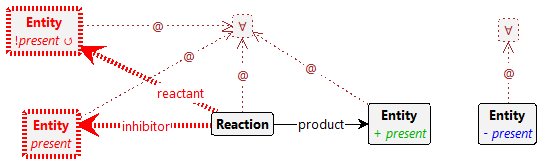
\includegraphics[scale=.42]{react}
\caption{Rule for reactions firing}
\label{fig:reactionfiring}
\end{figure}

The core rule describes the simultaneous firing of all \blab{Reaction}s of which no \lab{inhibitor}s and all \lab{reactant}s are present; the firing results in the presence of all \lab{product}s. Simultaneously, all currently present \blab{Entity}s are removed. In \GROOVE syntax, the core rule is drawn as in \Cref{fig:reactionfiring}.
To parse this, note that (in the \GROOVE notation) the red structure must be absent for the rule to apply; moreover, green labels are added and blue ones deleted upon rule application. The \ilab{present} flag signals whether an \blab{Entity} is considered to be currently present; hence, creating or deleting that flag comes down to creating or deleting the \blab{Entity}. The $\forall$-nodes impose the desired quantification, causing a single application of this rule to model the firing of all enabled \blab{Reaction}s, even if there are thousands of them.
Similarly for the simultaneous deletion of all \blab{Entity}s.

Our model also supports environments that inject \blab{Entity}s in a controlled manner. This is achieved by encoding the context specification in the initial graph and exploiting a second predefined rule, not shown here (see \Cref{fig:context}). A configuration is reachable if it can be constructed by the alternating application of both rules: first the context produces a set of stimuli (possibly upon inspection of the current state, but also nondeterministically or a combination of both), and then all enabled reactions are executed.

After a brief account of RSs (\Cref{sec:RS}) and \GROOVE (\Cref{sec:GTS}), we present the overall rationale, blueprint and key features of our approach in \Cref{sec:RS2GTS} through a simple vending machine example (\Cref{sec:student}).
The subsequent experimentation in \Cref{sec:experiments} is concerned with revisiting existing RS case studies to assess how \GROOVE can enhance their analysis. 
In particular, we tackle 
the comorbidity treatment scenario from~\cite{DBLP:conf/cmsb/BowlesBBFGM24} in \Cref{sec:cmsb2024}, 
the protein signalling networks analysis from~\cite{DBLP:conf/cmsb/BallisBFO24} in \Cref{sec:ccReact}, and
the T cell differentiation study from~\cite{datamod2023} in \Cref{sec:datamod2023}.
Our results are encouraging: \GROOVE is capable to explore large RSs 
%is well beyond what other tools have been able to achieve, 
by using roughly one tenth of the time compared to \BioResolve for both reachability and causal analyses.
More precisely, we are able to find a trace towards unwanted patterns (if they exist) among hundreds of thousands of reachable configurations using different heuristics; then, we can also prune the trace to extract a graphical representation of the causal history of that entities. Using the built-in model checker it is also possible to confirm the results of previous studies, as well as proving new facts.
A comparison with related tools is drawn in \Cref{sec:related}. Concluding remarks and future directions are discussed in \Cref{sec:conc}.


\section{Background}
% !TEX root =  ./main.tex

\subsection{RSs with Guarded Contexts}\label{sec:RS}

First, we briefly account for the classical set theoretic definition of Reaction Systems (RSs)~\cite{DBLP:journals/fuin/EhrenfeuchtR07}. Then, we focus on their process algebraic version~\cite{DBLP:journals/tcs/BrodoBF21} and its further extension with guarded contexts in~\cite{DBLP:conf/cmsb/BowlesBBFGM24} that are supported by the RS analysis framework \BioResolve.\footnote{\url{https://www.di.unipi.it/~bruni/LTSRS/}}


\subparagraph*{RS basics.}
A Reaction System is a pair ${\cal A} = (S, A)$, where $S$ is the finite set of \emph{entities}, and $A$ is a finite set of \emph{reactions} of the form $a = (R,I,P)$, with $R, I, P\subseteq S$ and $R \cap I = \varnothing$. 
The sets $R, I, P$ are the sets of \emph{reactants}, \emph{inhibitors}, and  \emph{products}, respectively. 
Without loss of generality, we admit the use of empty sets as reactants, inhibitors, and products.
%
Given the current state $W\subseteq S$, a reaction $a = (R,I,P)$ is enabled in $W$ if all its reactants are present (i.e., $R\subseteq W$) and all its inhibitors absent (i.e., $W \cap I = \varnothing$).
The \emph{result} of the reaction $a$ on the current state $W$ is $P$ if $a$ is enabled, and
$\varnothing$ otherwise.
The result of all reactions $A$ on the current state $W$, is the union of the results of all reactions.
%
The no-permanency principle of RSs dictates that entities disappear if not sustained by some reaction.
Thus, the current state $W=D\cup C$ is determined by the result $D$ of all reactions on the previous state, together with some additional entities $C$ that can be provided by the \emph{context} at each step. 

\subparagraph*{Process algebraic RSs and guarded contexts.}
Inspired by Plotkin's Structural Operational Semantics approach~\cite{DBLP:journals/jlp/Plotkin04a} and process algebras such as CCS~\cite{Milner80}, the key features of the process algebraic version of RSs are compositionality and the ability to account for a quite general notion of context (guarded, nondeterministic, recursive) using a friendly syntax. This way, we derive a Labelled Transition System (LTS) semantics for RSs by means of inductive inference rules, where LTS states are terms of an algebra, each transition defines a computation step of the RS and its label records the entities involved in that step.

\begin{definition}[RS processes]\label{def:LTSforRS}
%Let $S$ be a set of entities. 
\emph{RS processes} are defined by the grammar below:
\begin{eqnarray*}
\mathsf{P} & := & [\mathsf{M}]
\\
\mathsf{M} & := & (R,I,P) \mid D \mid \mathsf{K} \mid \mathsf{M}|\mathsf{M}
\\
\mathsf{K} & ::= & \nil \mid (R,I,C).\mathsf{K} \mid \mathsf{K}+\mathsf{K} \mid X
\end{eqnarray*}

\noindent
where $R$, $I$, $P$, $C$, and $D$ are sets of entities (with $R\cap I=\varnothing$) and $X$ is a context identifier drawn from a family of (recursive) definitions $\Delta \triangleq\{X_j=\mathsf{K}_j\}_{j\in J}$, called the \emph{environment}.
\end{definition}

Roughly, a RS process  $\mathsf{P}$ embeds a \emph{mixture} process $\mathsf{M}$ obtained as the parallel composition of some reactions $(R,I,P)$, some available entities $D$ (if any), and some \emph{context} process $\mathsf{K}$.
%We write $\prod_{i\in I} \mathsf{M}_i$ for the parallel composition of all $\mathsf{M}_i$ with $i\in I$. 
A  context process $\mathsf{K}$ is either: 
the nil context $\nil$ that stops the computation;
the guarded context $(R,I,C).\mathsf{K}$ that makes the entities $C$ available to the reactions if the reactants $R$ are present and the inhibitors $I$ are absent, and then will behave as $\mathsf{K}$ at the next step;
the non-deterministic choice $\mathsf{K}_1+\mathsf{K}_2$ that can behave as either  $\mathsf{K}_1$ or $\mathsf{K}_2$;  
the context identifier $X$ that behaves as $\mathsf{K}$ for $X=\mathsf{K}\in \Delta$.
We write $C.\mathsf{K}$ as a shorthand for the trivially guarded process $(\varnothing,\varnothing,C).\mathsf{K}$ and we assume the recursive context $\mathsf{Emp}=\varnothing.\mathsf{Emp}$ is always defined.


We say that $\mathsf{P}$ and $\mathsf{P}'$ are structurally equivalent, written $\mathsf{P} \equiv \mathsf{P}'$, when they denote the same term up to the laws of Abelian monoids (unit, associativity and commutativity) for  parallel composition $\cdot | \cdot$, with $\varnothing$ as the unit, and the laws of idempotent Abelian monoids for choice $\cdot +\cdot$, with $\nil$ as the unit. We also assume $D_1 | D_2 \equiv D_1\cup D_2$ for any $D_1,D_2\subseteq S$.
Indexed sums and parallel compositions are denoted, respectively, by $\sum_{i\in I} \mathsf{K}_i$ and $\prod_{i\in I} \mathsf{M}_i$.

The SOS semantics of  RS processes is defined by the SOS rules in \Cref{fig:guardforRS2nd}.
A transition label $\ell$, written $\obs{\obs{D}{R',I',C}}{R,I,P}$, records:
the available entities $D$; the entities $C$ provided by the guarded contexts, assuming all entities in $R'$ are present and those in $I'$ are absent;
the set $R$ of entities whose presence enables or disables some reactions;
the set $I$ of entities whose absence  enables or disables some reactions;
and the set $P$ of reaction products.
The  rules guarantee that, whenever $\mathsf{P}\xrightarrow{\obs{\obs{D}{R',I',C}}{R,I,P}} \mathsf{P}'$, it holds that $(R',I',C)$ is enabled in $D$ and that
$(R,I,P)$ is enabled in $W\triangleq (D\cup C)$.

\begin{figure*}[t]
		$$  
		\infer[(\textit{\scriptsize{Ent}})]
		{D \xrightarrow{\obs{\obs{D}{\varnothing,\varnothing,\varnothing}}{\varnothing,\varnothing,\varnothing}}\varnothing}
		{}
		\qquad\qquad
		\infer[(\textit{\scriptsize{Cxt}})]
		{(R,I,C).\mathsf{K} \xrightarrow{\obs{\obs{\varnothing}{R,I,C}}{\varnothing,\varnothing,\varnothing}}\mathsf{K}}{}
		$$
		\smallskip
		$$
		\infer[(\textit{\scriptsize Suml})]
		{\mathsf{K}_1 + \mathsf{K}_2 \xrightarrow{\ell}\mathsf{K}'_1}
		{\mathsf{K}_1 \xrightarrow{\ell}\mathsf{K}'_1}
		\qquad\qquad
		\infer[(\textit{\scriptsize Sumr})]
		{\mathsf{K}_1 + \mathsf{K}_2 \xrightarrow{\ell}\mathsf{K}'_2}
		{\mathsf{K}_2 \xrightarrow{\ell}\mathsf{K}'_2}
		\qquad\qquad
		\infer[(\textit{\scriptsize Rec})]
		{X \xrightarrow{\ell}\mathsf{K}'}
		{X=\mathsf{K}\in\Delta & \mathsf{K} \xrightarrow{\ell}\mathsf{K}'}
		$$
		\smallskip
		$$
		\infer[(\textit{\scriptsize Pro})]
		{(R,I,P)  \xrightarrow{\obs{\obs{\varnothing}{\varnothing,\varnothing,\varnothing}}{R,I,P}}(R,I,P)|P}
		{}
		\qquad\qquad
		\infer[(\textit{\scriptsize Inh})]
		{(R,I,P)  \xrightarrow{\obs{\obs{\varnothing}{\varnothing,\varnothing,\varnothing}}{J,Q,\varnothing}}(R,I,P)}
		{J \subseteq I & Q \subseteq R & J\cup Q\neq \varnothing}
		$$
		\smallskip
		$$
		\infer[(\textit{\scriptsize Par})]
		{\mathsf{M}_1~|~\mathsf{M}_2\xrightarrow{\ell_1\cup\ell_2} \mathsf{M}'_1~|~\mathsf{M}'_2}
		{\mathsf{M}_1 \xrightarrow{\ell_1} \mathsf{M}'_1 &
		\mathsf{M}_2 \xrightarrow{\ell_2} \mathsf{M}'_2 &
			\ell_1\frown \ell_2 }
		\qquad\qquad
		\infer[(\textit{\scriptsize Sys})]
		{[\mathsf{M}]\xrightarrow{\obs{\obs{D}{R',I',C}}{R,I,P}} [\mathsf{M}']}
		{\mathsf{M}\xrightarrow{\obs{\obs{D}{R',I',C}}{R,I,P}} \mathsf{M}' &
		R'\subseteq D &
        R\subseteq D\cup C}
		$$

\medskip	
\noindent
{\footnotesize
		where $\ell_1 \frown \ell_2$ and $\ell_1 \cup \ell_2$ are defined as follows:
		$$\begin{array}{l}
\obs{\obs{D_1}{R'_1,I'_1,C_1}}{R_1,I_1,P_1}
\frown
\obs{\obs{D_2}{R'_2,I'_2,C_2}}{R_2,I_2,P_2}
\\
\qquad\qquad\qquad\qquad\qquad\qquad\qquad\qquad\qquad\qquad\qquad\qquad\qquad
\triangleq (\textstyle\bigcup_{i=1,2} D_i\cup  R'_i) \cap (I'_1 \cup I'_2) = \varnothing
\wedge
(\bigcup_{i=1,2} D_i\cup  C_i\cup  R_i) \cap (I_1 \cup I_2) = \varnothing \\[5pt]
\obs{\obs{D_1}{R'_1,I'_1,C_1}}{R_1,I_1,P_1}
\cup
\obs{\obs{D_2}{R'_2,I'_2,C_2}}{R_2,I_2,P_2}
\\
\qquad\qquad\qquad\qquad\qquad\qquad\qquad\qquad\qquad\qquad\qquad\qquad\qquad
\triangleq \obs{\obs{D_1\cup D_2}{R'_1\cup R'_2,I'_1\cup I'_2,C_1\cup C_2}}{R_1\cup R_2,I_1\cup I_2,P_1\cup P_2}
\end{array}$$
}
		\caption{SOS semantics of the RS processes.}
		\label{fig:guardforRS2nd}
\end{figure*}


The rule $(\textit{Ent})$ records the set of current entities $D$.
By rule $(\textit{Cxt})$, a guarded context process $(R,I,C).\mathsf{K}$ makes available the entities in $C$ if the reactants $R$ are present in the current state and the inhibitors $I$ are absent, and then reduces to $\mathsf{K}$. 
Rules $(\textit{Suml})$ and $(\textit{Sumr})$ select a move of either the left or the right context, resp., discarding the other process.
By rule $(\textit{Rec})$, a context identifier $X$ behaves according to its defining process $\mathsf{K}$.

The rule $(\textit{Pro})$ assumes the reaction $(R,I,P)$ is enabled: it records its reactants, inhibitors, and products in the label, and leaves the reaction  available at the next step, together with its products $P$.
The rule $(\textit{Inh})$ records in the label the reasons why the reaction $(R,I,P)$ should not be executed: possibly some inhibiting entities $(J \subseteq I)$ are present or some reactants $(Q \subseteq R)$ are missing, with $J \cup Q \neq \varnothing$, as at least one cause is needed.

The rule $(\textit{Par})$ puts two processes in parallel by pooling their labels and joining all labels components. We write $\ell_1\cup\ell_2$ for the component-wise union of labels, while the sanity check $\ell_1\frown\ell_2$ is required to guarantee that labels of reactants and inhibitors are consistent (see definitions in \Cref{fig:guardforRS2nd}).

Finally, the rule $(\textit{Sys})$ checks that all the needed reactants are available in the system. Checking the absence of inhibitors  is not necessary, thanks to the sanity check in rule $(\textit{Par})$.
Note that, while the enabling of $(R,I,C).\mathsf{K}$ requires the presence of reactants $R$ and the absence of inhibitors $I$ w.r.t. the set of current entities $D$, in the case of reactions $(R,I,P)$, the check is performed w.r.t. the current state $W=D\cup C$.
More importantly, the products $C$ are made available immediately from the context, not at the next step.
It is worthy to mention that a conditional prefixed process that is not enabled behaves as the $\nil$ process.

A first concrete example of RS that exposes most features is presented in \Cref{sec:student}.


% !TEX root =  ./main.tex

\subsection{GT and GROOVE}\label{sec:GTS}

Graph Transformation (GT, sometimes called Graph Rewriting) is a well-established rule-based formalism, the core of which is to specify precisely how graphs may evolve. Each rule embodies a particular change, which can be applied to a given graph (in the simplest form consisting of nodes and binary edges) by establishing where in that graph the preconditions of the rule are met, and then adding and deleting nodes and edges as prescribed.

In this paper, we use the so-called \emph{algebraic approach} to graph transformation (see \cite{DBLP:series/eatcs/EhrigEPT06} for a formal exposition and \cite{DBLP:books/sp/HeckelT20} for applications in the context of software engineering); moreover, we rely on the particular flavour implemented in the tool \GROOVE \cite{DBLP:journals/sttt/GhamarianMRZZ12,GROOVE}. Some of the relevant features of the approach and the tool are highlighted below.

\textbf{Graphs} are \emph{simple} and \emph{typed}, meaning that there is at most one edge of a given type between any two nodes and that all nodes and edges are labelled through a morphism to a given (fixed) \emph{type graph}. Edges are \emph{directed} (going from their \emph{source} to their \emph{target}). Besides binary edges, nodes can also have \emph{flags} (which are actually self-loops that act as additional, optional labels on nodes) and \emph{attributes} (which are actually binary edges whose target node is a data value, e.g., an integer or a string).

\textbf{Rules}, in their simplest form, consist of a left hand side (LHS) and right hand side (RHS). Rule applicability is established by \emph{matching} the LHS to the graph in question, and where a match exists, removing nodes and edges that are in the LHS but not in the RHS, and vice versa, adding nodes and edges that are in the RHS but not in the LHS. In addition, however, \GROOVE supports \emph{quantified} rules, which can simultaneously be applied to multiple places in the same graph. An example is shown in \Cref{fig:context} below.

\textbf{Evolution} of a graph is defined on the basis of a graph transformation \emph{system}, which is a set of rules applied to a graph at hand, giving rise to a modified graph to which every rule can be applied again, and so forth. On top of this, \GROOVE allows for \emph{control programs} that can specify in what order rules may be applied. By exploring the potential evolution of a graph in all ways allowed by the control program, \GROOVE constructs the \emph{state space} of the graph transformation system, in the form of a \emph{labelled transition system} consisting of all reachable graphs and the rule applications between them.

\textbf{Analysis} consists of the exploration of the state space for a given initial graph, rule system and (optional) control program. The exploration can be tuned by built-in strategies for searching and model checking.
%\todo{RB: slightly rearranged}
%The core functionality of \GROOVE is to explore the set of reachable graphs, given a graph transformation system (with or without control program) and an initial graph. With this as the basis, there are built-in strategies for searching and model checking.

\smallskip\noindent
The power of graph transformation lies in its generality: many systems naturally lend themselves to be modelled as graphs, and algebraic rules --- especially quantified ones --- provide a rich framework to specify their evolution. This is in fact our motivation for using it the current paper: reaction systems can straightforwardly be interpreted as graphs. \Cref{fig:core-type} shows the core types for the relevant concepts of that interpretation. (The colours just support the visualisation and have no semantics of their own.)

\begin{figure}
\centering
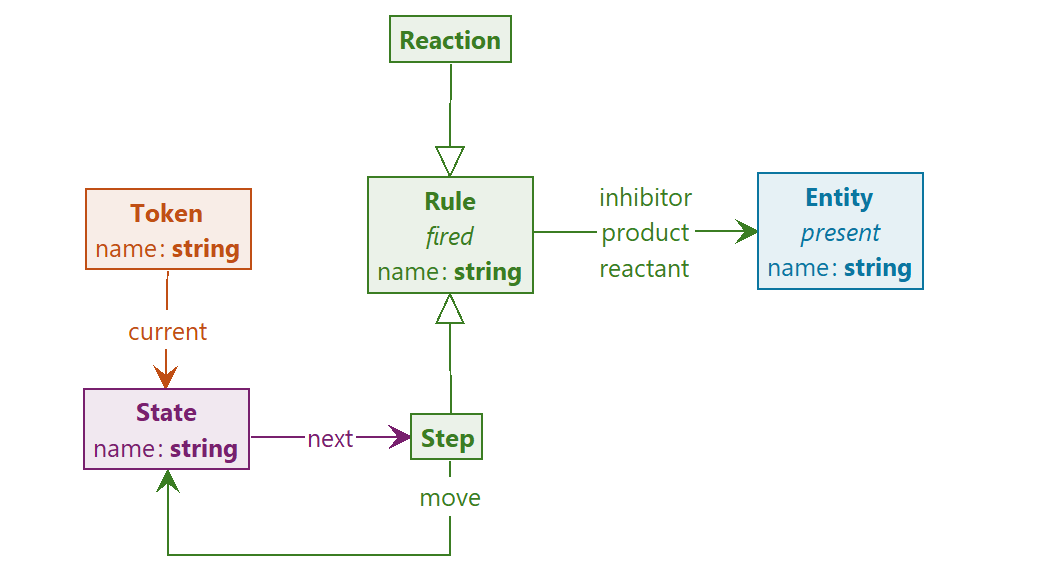
\includegraphics[scale=.5]{figs/core-type}
\caption{Core type graph for reaction systems}
\label{fig:core-type}
\end{figure}
%
Note especially the (abstract) supertype \Rule with subtypes \Reaction and \Step: the former is the type for the elements of $A$ in a Reaction System ${\cal A}=(S,A)$, whereas the latter is used to represent triples $(R,I,P)$ in a context RS process. The flag \fired is used to mark \Rule{}s that have triggered in the most recent step. The set $S$ is represented by nodes of type \Entity; for a given \Rule, the subsets $R$, $I$, and $P$ of $S$ are those \Entity{}s to which there is an outgoing edge labelled \reactant, \inhibitor or \product. The subtype \Forbidden anticipates the principle, demonstrated later in this paper, of identifying undersirable entities and specifically searching for scenarios in which those are produced. The flag \present is used to label the entities occurring in a state $W$. Finally, the structure of (guarded) context processes is captured by \State entities, with \nextt-edges to the \Step{}s that can be nondeterministally chosen; the subsequent process after such a \Step is determined by its outgoing \move-edge. \Token nodes are used to model which \State{}s are currently active.



% !TEX root =  ./main.tex

\section{Toy Example}\label{sec:student}

To illustrate some basic concepts of RSs and, in the next section, of the proposed encoding, we model a system composed of a student and a vending machine as a toy example.
The vending machine accept two different kinds of coins and can dispense either a cappuccino or an expresso when a coffe coin is inserted or a tea if a tea coin is inserted. A cappuccino is dispensed if some milk is available, otherwise the expresso is produced.
Assuming the powder for preparing coffee and tea are always present, the corresponding process can be written as follows:
\[
\begin{array}{lll}
\mathsf{VM} & \triangleq & (\{\ccoin,\cpowder\},\{\nomilk\},\{\cappuccino\})\\
& | & (\{\ccoin,\cpowder,\nomilk\},\emptyset,\{\espresso\})\\
& | & (\{\tcoin,\tpowder\},\emptyset,\{\tea\})\\
& | & (\{\cpowder\},\emptyset,\{\cpowder\})\\
& | & (\{\tpowder\},\emptyset,\{\tpowder\})\\
\end{array}
\]

A refill context process can, nondeterministically, refill the machine with milk.
\[
\begin{array}{lll}
\mathsf{Refill} & \triangleq & \{\nomilk\}.\mathsf{Refill}\\
& + & \emptyset.\mathsf{Refill}\\
\end{array}
\]

The student process is very simple: she takes cappuccino in the morning and tea in the afternoon, otherwise she gets angry.
\[
\begin{array}{rll}
\mathsf{Student} & \triangleq & (\emptyset,\{\am\},\{\tcoin\}).\mathsf{GetTea}\\
& + & (\{\am\},\emptyset,\{\ccoin\}).\mathsf{GetCappuccino}\\
& + & \{\idle\}.\mathsf{Student}\\
\mathsf{GetCappuccino} & \triangleq & (\{\cappuccino\},\emptyset,\emptyset).\mathsf{Student}\\
& + & (\{\espresso\},\emptyset,\{\anger\}).\mathsf{Student}\\
\mathsf{GetTea} & \triangleq & (\{\tea\},\emptyset,\emptyset).\mathsf{Student}\\
& + & (\emptyset,\{\tea\},\{\anger\}).\mathsf{Student}\\
\end{array}
\]

Finally, two more reactions model the passage of time (morning vs afternoon) while the student is idle.
\[
\begin{array}{lll}
\mathsf{Day} & \triangleq & (\{\idle\},\{\am\},\{\am\})\\
& | & (\{\am\},\{\idle\},\textcolor{red}{\{\am\}})
\end{array}
\]

We assume that, initially, both entitites $\cpowder$ and $\tpowder$ are present.
So the system can be written as:
\[
[\,\{\cpowder,\tpowder\} 
| \mathsf{VM}
| \mathsf{Refill}
| \mathsf{Day}
| \mathsf{Student}
\,]
\]

Using BioReSolve, we can generate the underlying LTS as in Fig.~\ref{fig:toylts}: the initial state is in light blue, while the state where the student is angry is in light coral.

\begin{figure}
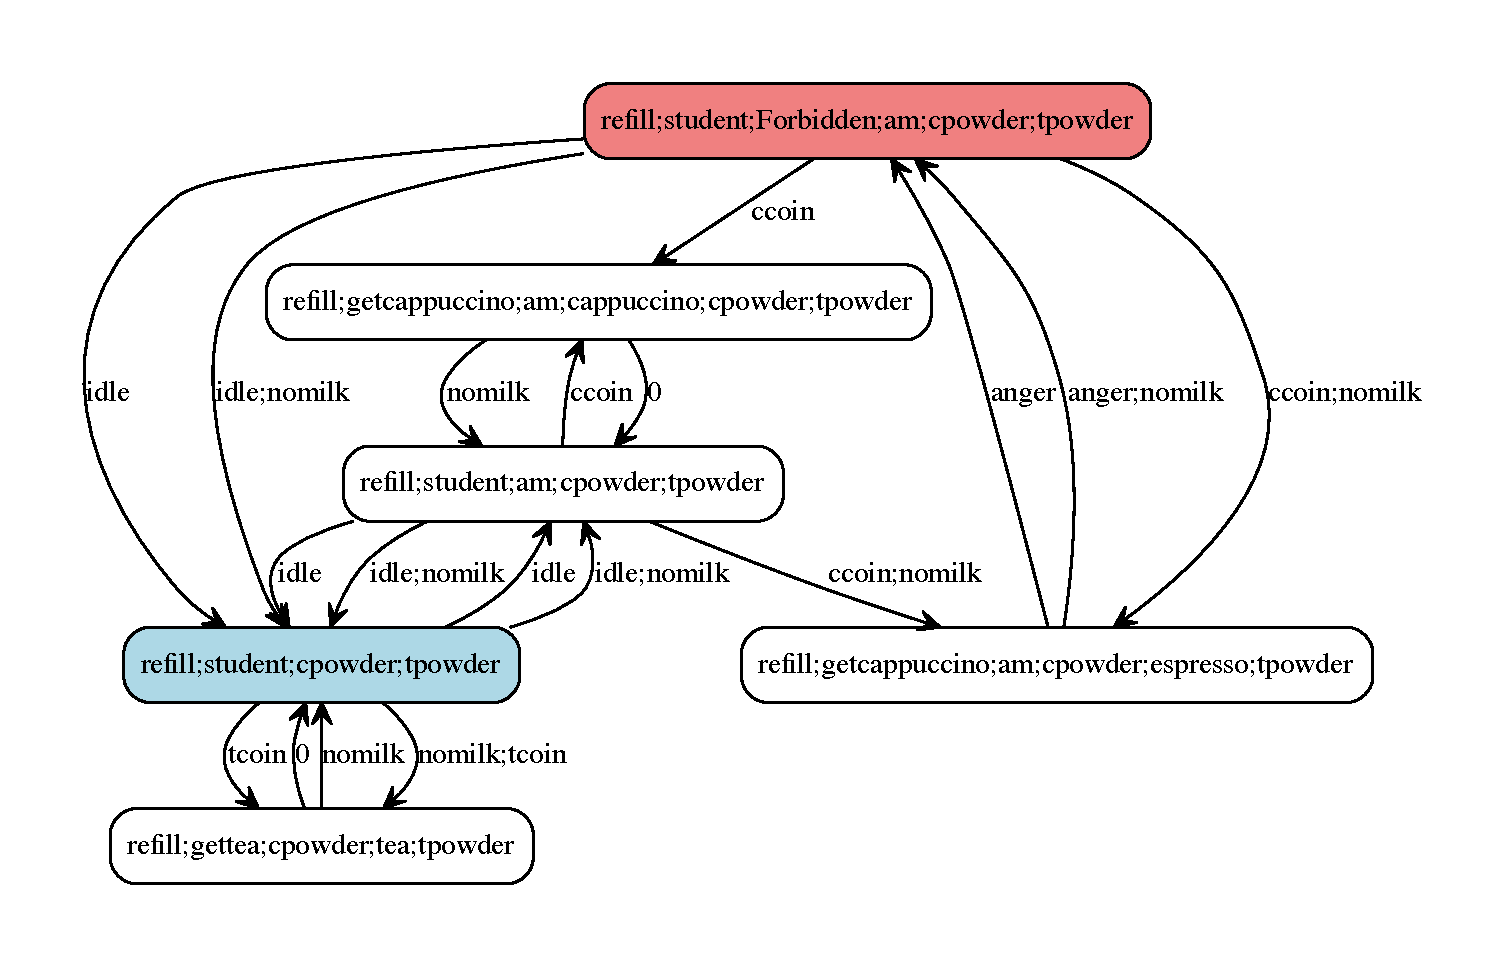
\includegraphics[scale=.3]{toylts}
\caption{LTS of the toy example.}\label{fig:toylts}
\end{figure}

% !TEX root =  ./main.tex

\section{Encoding of RS in GT}\label{sec:RS2GTS}

As an alternative to BioResolve, we investigate the use of graph transformation and \GROOVE to generate the underlying LTS of a given Reaction System, on the basis of a start graph obtained by transformation from the RS specification. Because the start graph will typically include special \Entity subtype, it comes together with an additional type graph where those are specified. Depending on what one wants to analyse, the various strengths and capabilities of \GROOVE then come into play.

For instance, one possibility is to use \GROOVE's model checking capabilities to check for temporal patterns of entity generation in the transition system. Another way to proceed is to focus on a given trace and build its \emph{occurrence graph}, which contains all the rule occurrences and entity instances present in that trace --- analogous, in fact, to the way a Petri net process captures a particular behaviour. If the trace in question leads to a state in which a forbidden entity is present (such as the $\bang$ entity in our toy example), we can also \emph{prune} the occurrence graph, again using graph transformation, to keep only those rule occurrences and entity instances that directly contributed to the existence of the forbidden entity.

This gives rise to the tool chain depicted in \Cref{fig:chain}, the phases of which will be explained in some more detail in the remainder of this section.	

\begin{figure}
\centering
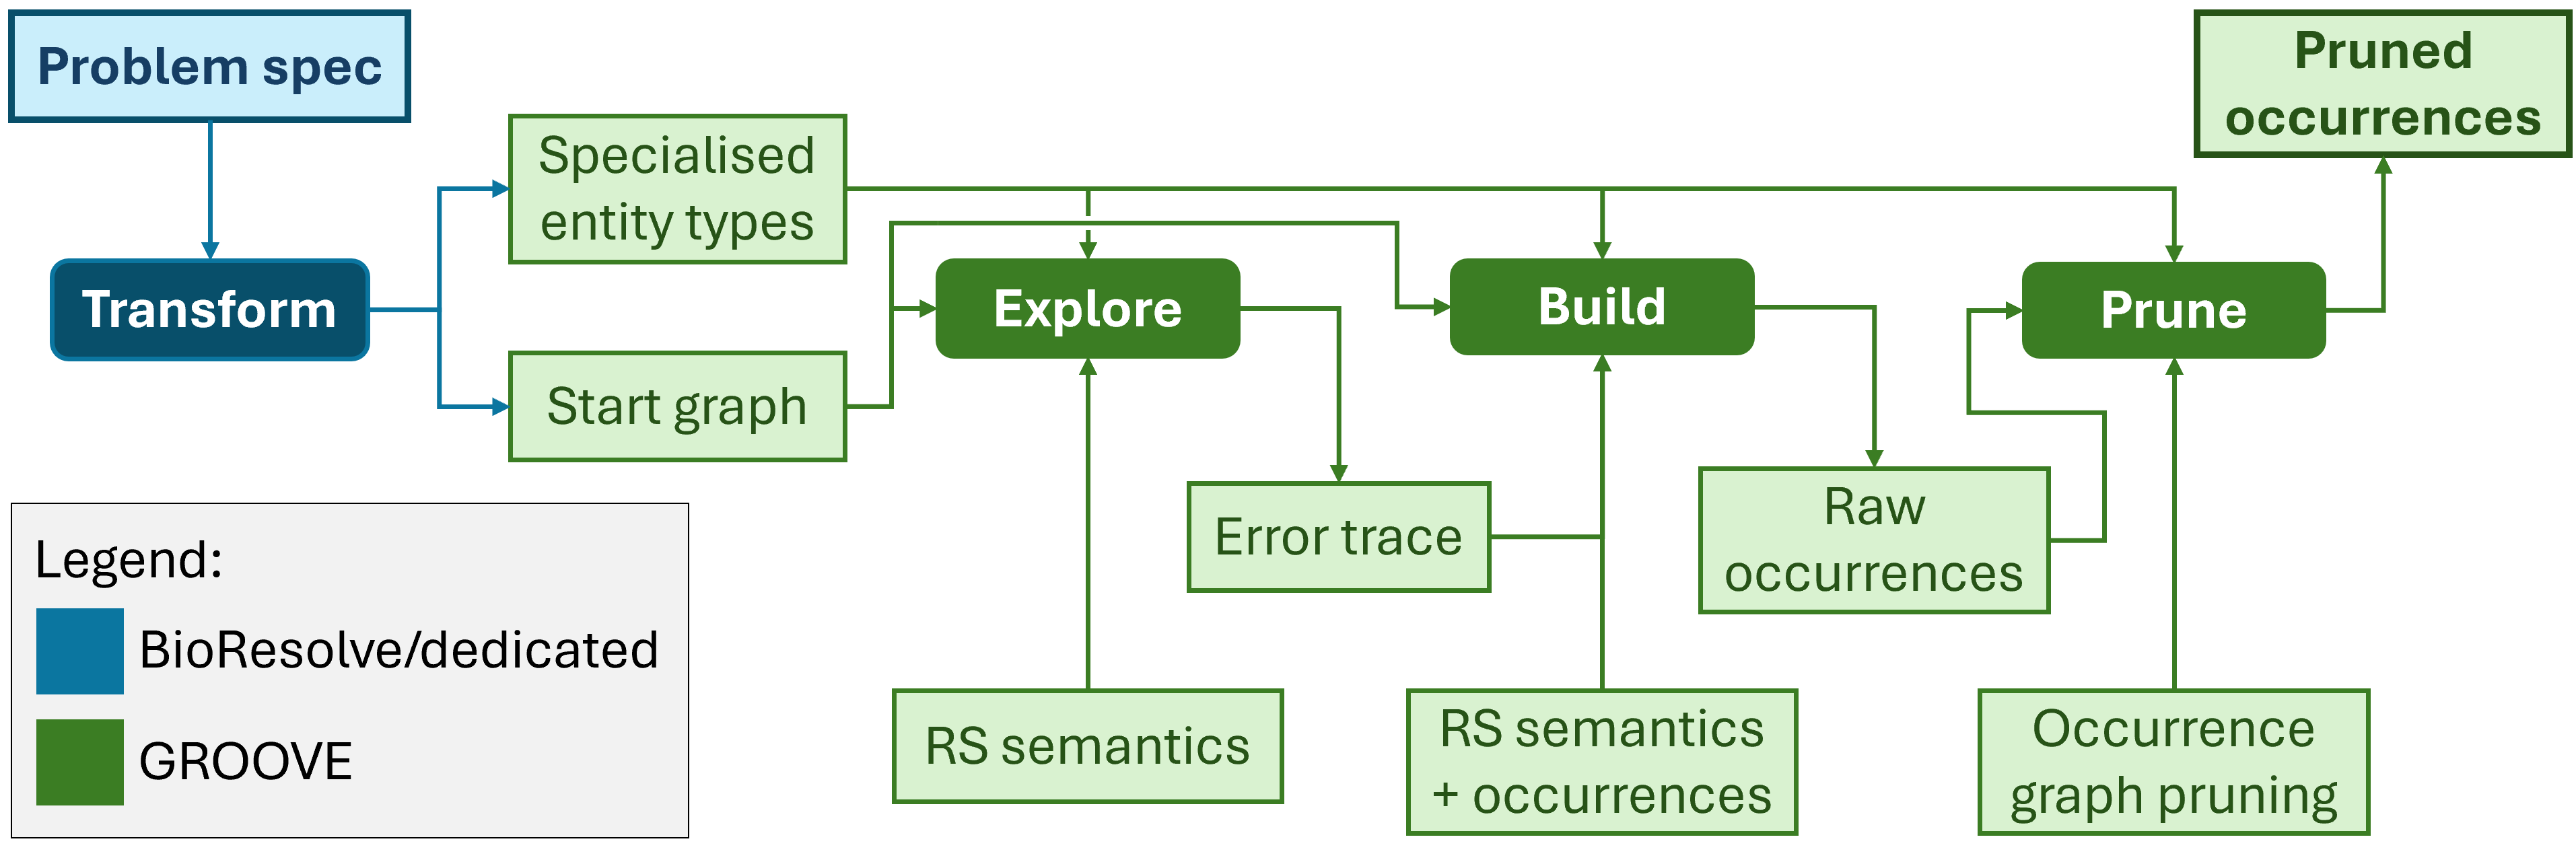
\includegraphics[scale=.25]{figs/chain}
\caption{Reaction System exploration and analysis using \GROOVE}
\label{fig:chain}
\end{figure}

\medskip\noindent\textbf{Transform.}
%
The first step is a text-to-model transformation from a problem specification in \BioResolve syntax into \GROOVE syntax. This is achieved by running the \verb=main_do(rs2gts)= directive of \BioResolve, which produces two artifacts: firstly, an additional type graph, complementary to the one shown in \Cref{fig:core-type}, which specifies subtypes of \Entity for all entities in the problem at hand (essentially for performance reasons: relying on dedicated types speeds up the matching step of \GROOVE); and secondly (more importantly) a start graph in which the entire \BioResolve system is encoded as suggested by \Cref{fig:core-type}. For the example system, the additional types as well as two self-explanatory fragments of the start graph are shown in \Cref{fig:toy}.

\begin{figure}
\centering
\subcaptionbox{Specialised entity types}{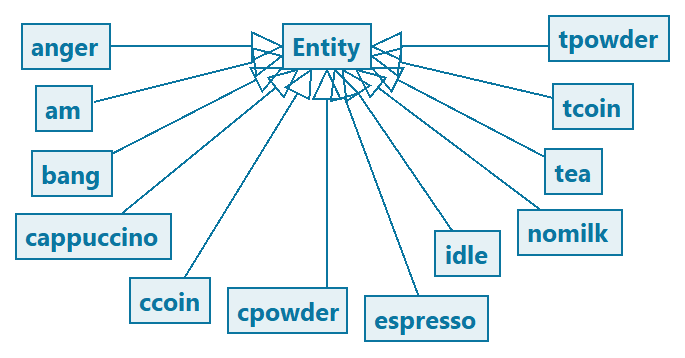
\includegraphics[scale=.2]{figs/toy-type}}
\subcaptionbox{Start graph fragment: Three reactions from $\mathsf{VM}$}{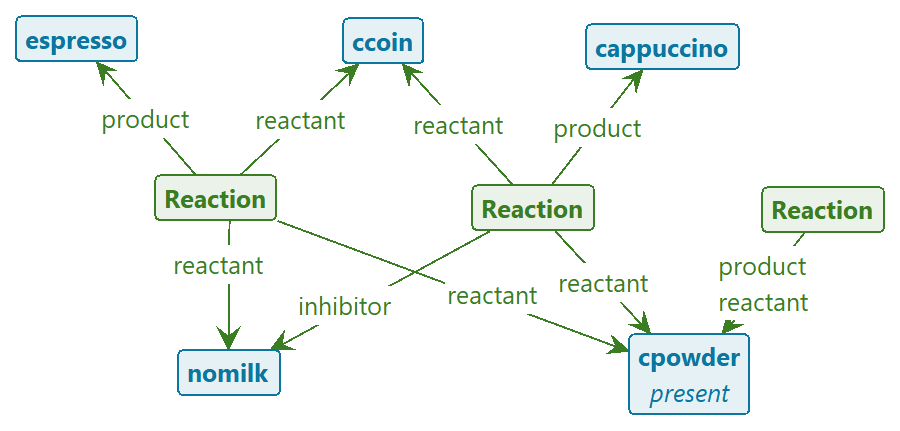
\includegraphics[scale=.2]{figs/toy-reactions}}
\subcaptionbox{Start graph fragment: The \textsf{Student} context process}{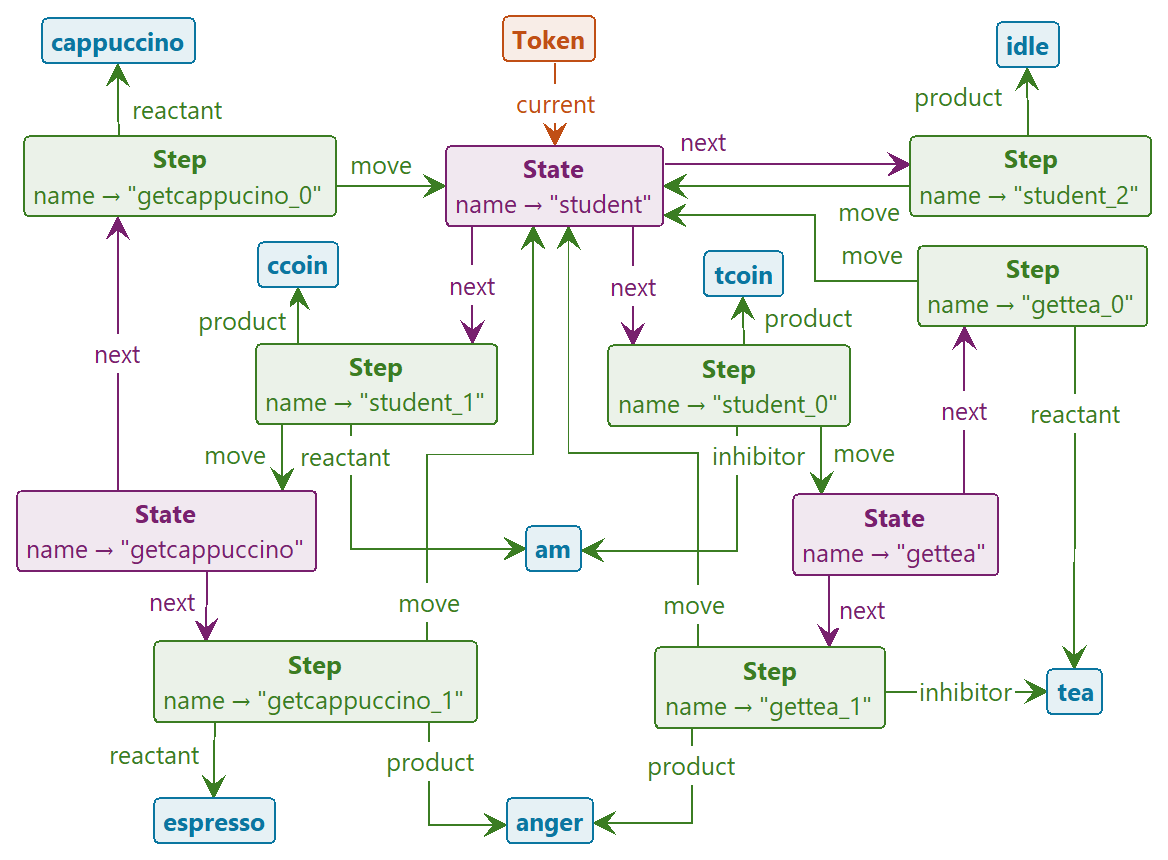
\includegraphics[scale=.2]{figs/toy-context-named}}
\caption{Graph representation of running example}
\label{fig:toy}
\end{figure}

\medskip\noindent\textbf{Explore.}
%
The dynamics of Reaction Systems is encoded as a combination of two rules, \contextR and \reactR, which are scheduled to fire in alternation. \contextR encodes the simultaneous firing of all context processes (nondeterministically selecting an enabled \Step from every \State with a \Token), whereas \reactR encodes the (deterministic) simultaneous firing of all enabled \Reaction{}s, while simultaneously erasing all \Entity{}s that were not just produced. The production or erasure of an \Entity is encoded through the creation or deletion of a \present flag on a (persistent) \Entity node, \emph{not} by the creation or deletion of the node itself. In addition, to keep track of which nondeterministic choices were actually taken, the \contextR rule marks the \Step{}s that were selected with a \fired flag, which is subsequently erased by the \reactR rule. % A third rule called \firedR (actually a \emph{condition}, which in \GROOVE is a rule that does not modify the graph) checks for the occurrences of the \fired flag and so exposes the names of the \Rule{}s that have fired in the transition system.

\begin{figure}
\centering
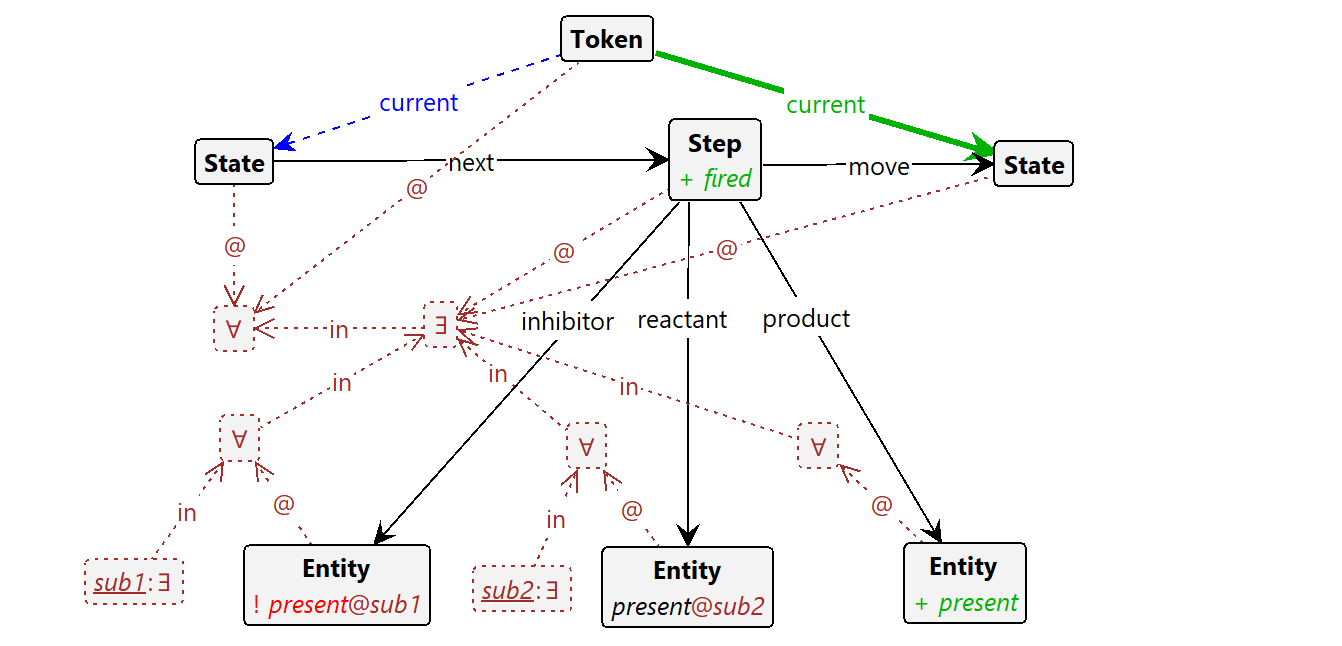
\includegraphics[scale=.2]{figs/context}
\caption{Rule for context firing}
\label{fig:context}
\end{figure}
%
\Cref{fig:context} shows the first (and most intricate) of these rules, viz.\ the one for the context firing. This is a quantified rule, which can be read as follows: \uline{For all} \State{}s with a \Token, \uline{there is} a \nextt{} \Step such that \uline{for all} \inhibitor{}s \uline{there is no} \present flag whereas \uline{for all} \reactant{}s \uline{there is} a \present flag; moreover, when the rule is applied, \uline{all} \product{}s of the selected \Step{}s receive a \present flag, the \Step{}s themselves receive a \fired flag, and all \Token{}s move to the successor \State{}s. Colour coding is used in the visual representation to distinguish the quantifier nodes $\forall$ and $\exists$ (both in purple), as well as the mandatory absence (red), deletion (blue) and creation (green) of edges and flags.\footnote{This colour coding is \GROOVE-specific and entirely separate from the problem-specific colouring of the graph nodes in Figures \ref{fig:core-type} and~\ref{fig:toy}; in fact, to avoid confusion, the problem-specific colouring is \emph{not} used in the rule view.}

To mimic the \BioResolve semantics as closely as possible, we can instruct \GROOVE to regard every pair of \contextR- and \reactR-transitions as an atomic transaction, corresponding precisely to a transition in \BioResolve (though not with the same label), and then generate the entire state space. This is achieved through a control program of the form
%
\begin{lstlisting}[keywordstyle=\bfseries,morekeywords={recipe}]
recipe fire() {
  context; react;
}
\end{lstlisting}
%
where a ``recipe'' is the keyword for a transaction wrapping the body. With this in place, the GUI-based version of \GROOVE produces the transition system displayed in \Cref{fig:toy-gts} (which can also be exported to a range of standard formats), which is easily (visually) checked to be essentially isomorphic to the one in \Cref{fig:toylts}.

\begin{figure}
\centering
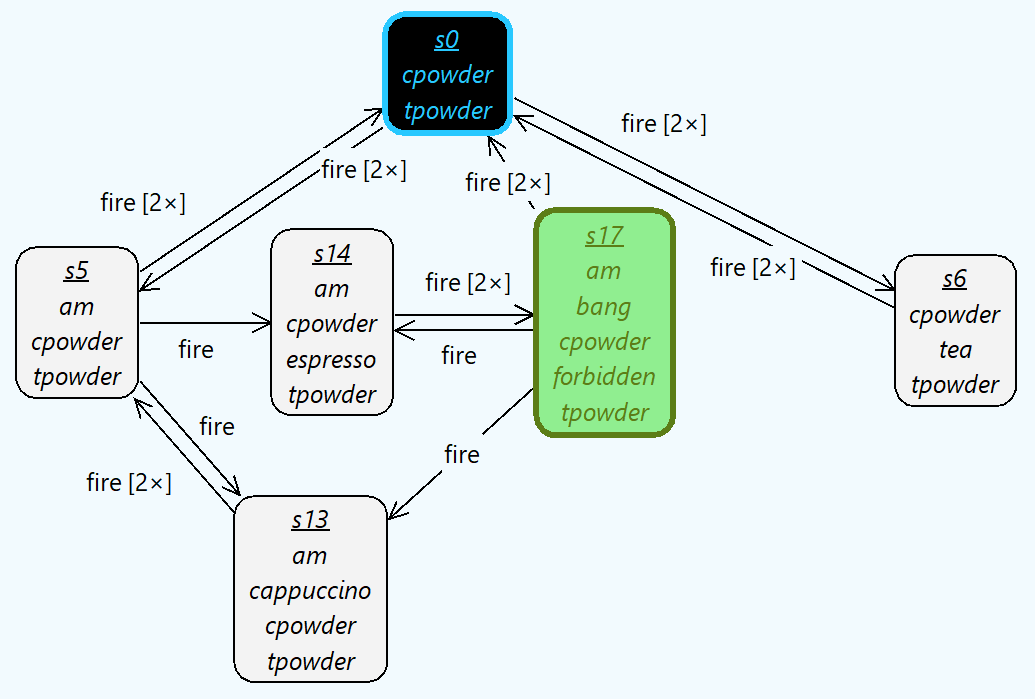
\includegraphics[scale=.2]{figs/toy-gts}
\caption{\GROOVE LTS of the toy example}
\label{fig:toy-gts}
\end{figure}

Alternatively, we can (for instance) ask \GROOVE to search the for the first reachable state in which the \Forbidden entity appears, using breadth-first search. (In fact, the state property for which \GROOVE searches is itself determined by a rule, which in this case merely tests for the presence of a \Forbidden entity). When found, the trace to the forbidden state can be saved as a control program that drives the next stage of \GROOVE exploration. In particular, using the alternating application of the \contextR and \reactR rules (rather than the transactional variant used for \Cref{fig:toy-gts}) this control program also records the \firedR-applications that tell which \Step{}s have fired: this completely determines how the non-determinism in the context process has been resolved in order to arrive at the forbidden state. Here is the control program for the shortest trace to state \textsf{\itshape s17} in our running example:

\begin{center}
\begin{lstlisting}
context;
fired("student_2");
fired("refill_1");
react;
context;
fired("student_1");
fired("refill_0");
react;
context;
fired("refill_1");
fired("getcappuccino_1");
react;
\end{lstlisting}
\end{center}
%
Here \textsf{student\_2}, \textsf{student\_1} and \textsf{getcappucino\_1} are the \Step{}s of the \textsf{Student} process visualised in \Cref{fig:toy}; \textsf{refill\_1} and \textsf{refill\_0} are the steps of the \textsf{Refill} process given in \Cref{sec:student}.

\medskip\noindent\textbf{Build.}
%
The purpose of this phase is to build an occurrence graph that explains how \Forbidden was produced, by collecting its (transitive) dependencies. Concretely, we record the following dependencies:\todo{Refer to literature}
\begin{itemize}
\item From each non-initial \Entity instance to the \Rule occurrence of which it is the \product;
\item From each \Rule occurrence to all its reactant \Entity instances;
\item From each \Step occurrence to all directly preceding \Step occurrences.
\end{itemize}
%
Note that this is restricted to \emph{positive} dependencies. In fact, we have constructed our example so that there are no inhibitors in the \Rule{}s that fire in the trace above; if we would rely on an entity \milk that inhibits the production of \espresso, rather than on \nomilk as a reactant, the occurrence graph for \bang would not include \milk; and likewise if we would use \cappuccino as an inhibitor for \anger rather than \espresso as a reactant for it. The representation of negative dependencies is a research question in its own, and is outside the scope of this paper;\todo{Refer to literature} \Cref{fig:occur-type} shows the occurrence type graph. 

\begin{figure}
\centering
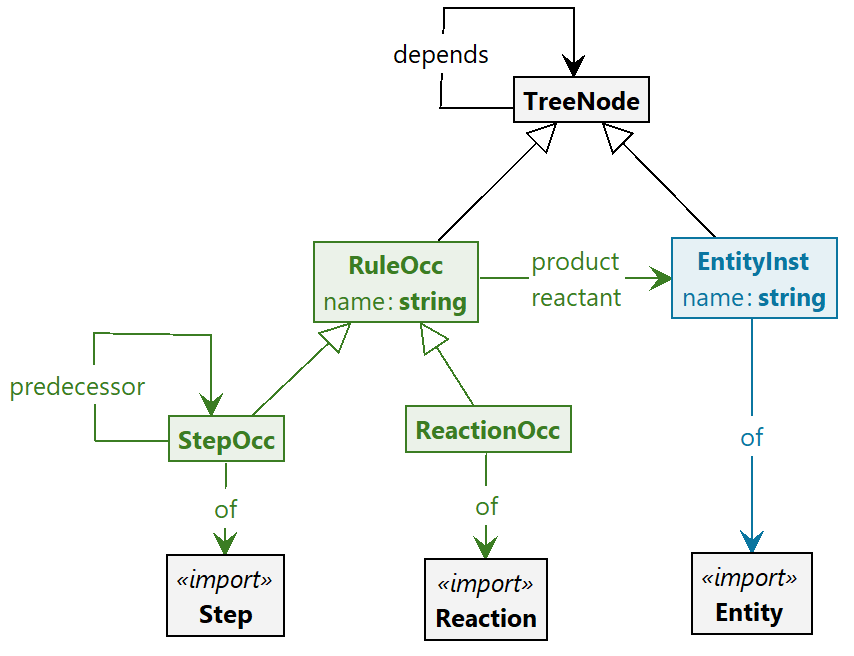
\includegraphics[scale=.2]{figs/occur-type}
\caption{Occurrence type graph}
\label{fig:occur-type}
\end{figure}

As indicated in \Cref{fig:chain}, the occurrence graph is produced by another \GROOVE rule system, using the same start graph but driven by the control program previously created in the explore phase, encoding (as we have seen) the trace to the undesirable state. The occurrence graph semantics consists of rules with the same names (\reactR, \contextR and \firedR), but different functionality: in particular, rather than manipulating \present flags, the \reactR rule now creates \RuleOcc- and \EntityInst-nodes together with their dependencies. This is a non-trivial procedure that in fact itself requires several successive stages. Though the details of these stages are not of sufficient interest to include in this paper, we want to point out that breaking down a single rule (\reactR, in this case) into multiple stages is opposed to the usual view, engrained in algebraic graph transformation, that a rule embodies a single, atomic change to a graph. This contradiction is solved by another feature of \GROOVE, namely \emph{recipes}. A recipe is a procedural control abstraction that has transactional semantics, and hence for the purpose of exploration acts just like an atomic rule; however, its body may consist of an arbitrary control (sub-)program. In the occurrence graph semantics, therefore, \reactR is actually not a rule but a recipe, defined as

\begin{center}
\begin{lstlisting}[basicstyle=\sffamily\small,columns=fullflexible,xleftmargin=1cm,keywords={recipe},literate={-}{-}1]
recipe react() {
  entities-age;
  react-produce;
  merge;
}
\end{lstlisting}
\end{center}
%
\medskip\noindent\textbf{Prune.}
%
Unfortunately, the occurrence graph built by the rule system described above is too large to be useful: it contains \emph{all} entities and rule occurrences produced by the trace, not just the dependencies of the undesired \Forbidden entity. Moreover, the entire start graph is also (still) present. Therefore, in a third phase, all redundant information is pruned. This is achieved by first marking all transitive backward dependencies of \Forbidden, and then removing all unmarked nodes. Since this is straightforward, and of no particular interest in the context of this paper, we omit the details of the \GROOVE rule system for this phase. Its outcome for our running example is shown in \Cref{fig:toy-pruned}.


\begin{figure}
\centering
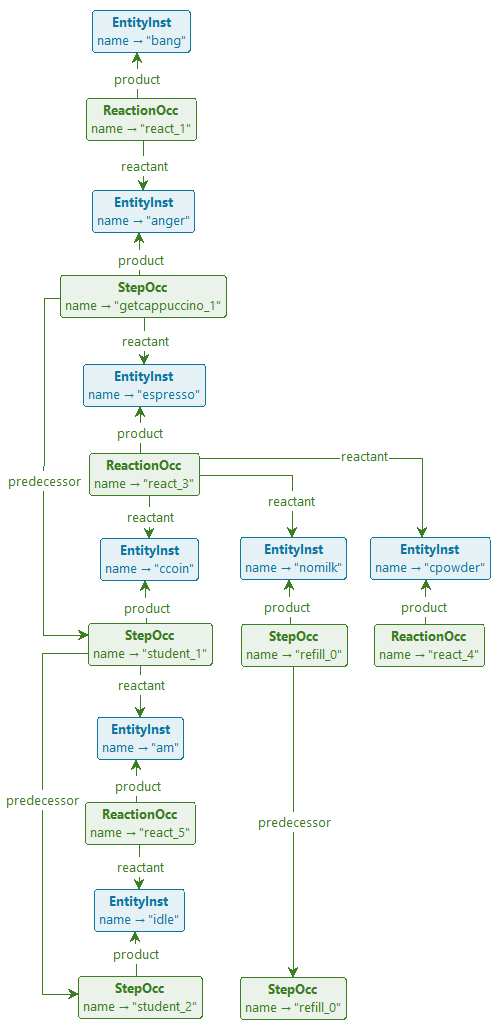
\includegraphics[width=\columnwidth]{figs/toy-pruned}
\caption{Pruned occurrence graph}
\label{fig:toy-pruned}
\end{figure}

The pruned occurrence graph visualises the causal effect chain already explained informally at the end of \Cref{sec:student}: the presence of a \ccoin, which itself depends on \am, combined with \cpowder and \nomilk causes the production of \espresso, after which the student produces \anger, which is \Forbidden.

\begin{comment}
\begin{quote}\it Notes:
\begin{itemize}
\item Rules for implementing RS semantics
\item Conversion of a trace to a control program
\item Using recipes in the occurrence graph building
\end{itemize}
\end{quote}
\end{comment}

% !TEX root =  ./main.tex

\section{Experimentation}\label{sec:experiments}

Here we consider 
three larger case studies whose RS specifications have already appeared in the recent literature. For each case study, we briefly describe its main features and then show how the methodology outlined in the previous sections can be applied for carrying out some fruitful experimentation with \GROOVE.

All \GROOVE experiments were carried out using \href{https://github.com/nl-utwente-groove/code/releases/tag/release-7_4_3}{\GROOVE version 7.4.3} on a Dell Precision 3551 laptop with an Intel i7 CPU running at 2.6 GHz; \GROOVE was run in a Java~24 JVM with 12GB of memory. No attempt was made to measure running time with precision, and repeated experiments have shown that the reported durations can deviate up to 25\%. In order to facilitate replication of the experiments, we have included supplementary materials with this paper, including the required rule systems and start graphs and instructions for invoking \GROOVE; see \Cref{app:groove}.


% !TEX root =  ./main.tex

\subsection{Comorbidity Treatment Analysis}

The paper~\cite{DBLP:conf/cmsb/BowlesBBFGM24} introduced the notion of RS with guarded contexts, as recalled in \Cref{sec:RS}.
%to model scenarios where the entities to be provided by the context are dependent upon the current state, which is a common situation arising, e.g., in drug administration and \emph{in silico} experiments. 
The motivating case study considered in~\cite{DBLP:conf/cmsb/BowlesBBFGM24} is the risk reduction of medication harm in the treatment of patients with comorbidities; i.e., patients with two or more long-term chronic conditions (such as diabetes, hypertension, cardiovascular diseases, chronic kidney disease, cancer, chronic obstructive pulmonary disease, among many others), who are therefore subject to follow several treatment plans simultaneously, called \emph{clinical guidelines}~\cite{feder1999using,woolf1999potential}. Since clinical guidelines address a single disease, comorbidities easily lead to  \emph{polypharmacy}, where 5 or more medications must be administered, increasing the risk of adverse drug reactions, or of making certain drugs less effective when combined~\cite{Gut12}. Using formal methods for risk mitigation intends to help doctors choose between alternative treatment options as well as to point out missing conditions that could be helpful to revise and update clinical guidelines. 

\subparagraph*{Features of interest.}
In this case study, reachability and causal analysis are key issues.
Specifically, reachability is used to address questions such as \emph{can the combination of clinical guidelines expose the patient at serious risks because of drugs interference?}
Then, in the affirmative case, causal analysis can help to detect which medical decisions would be directly responsible for causing serious harm as well as to point out  which alternative treatment would be available, if any.
We have selected this case study because the use of guarded contexts poses new challenges in terms of causal analysis: an external choice, apparently made by the context, might in fact be the only option available given the actual state of the system. \todo{A: I don't quite get it - what is the new challenge?}

\subparagraph*{Experimental set up.}
The RS encoding proposed in~\cite{DBLP:conf/cmsb/BowlesBBFGM24} relies on a formal representation of patient profiles, medical guidelines and adverse drug reactions.

For medical guidelines, it takes in input the event structure modelling of therapies introduced in~\cite{BC17c}. Roughly, to each event $e$ there is an identifier $\mathsf{E}_e$ defined as a sum of processes, one for each outgoing arc of $e$. If some guard is attached to the arc, then the corresponding alternative is also guarded. When some drug prescription for $d$ is present in a node, then the corresponding choice produces $\mathsf{get}\_d$. Similarly, if the therapy requires stopping some drug $d$, the entity $\mathsf{stop}\_d$ is produced.
Concurrent events are activated separately.\todo{This sentence is not clear to me.}

The patient profile is determined by the conditions that trigger the treatment (e.g., headache, hypertension) and by the conditions that appear in the arc labels of the event structure (e.g., pregnant, asthma). We call them \emph{features}. The patient profile is thus just a combination of features. Correspondingly, there is one context $\mathsf{K}_f = \emptyset.\mathsf{Empty} + \{f\}.\mathsf{Empty}$ for each feature $f$, and any possible combination of features is accounted for by their parallel composition $\prod_f \mathsf{K}_f$. Alternatively, specific profiles can be investigated by removing some alternatives from each $\mathsf{K}_f$.\todo{Why is this useful?}
Once the profile is determined by the context, it is preserved during the rest of the computation by reactions of the form $(\{f\},\emptyset,\{f\})$, one for each feature.

For each drug $d$ that appears in the therapies, we consider three corresponding entities $\mathsf{get}\_d$, $\mathsf{stop}\_d$  and $d$: the first represents the prescription of $d$ by the doctor, the second the removal of $d$ from the current treatment and the third the intake of the drug by the patient. 
Entities $\mathsf{get}\_d$ and $\mathsf{stop}\_d$ will be provided by the context that models the guideline, as discussed above. 
For each drug, $d$ there will be the following reactions: $(\{\mathsf{get}\_d\},\{\mathsf{stop}\_d,\mathsf{stop}\_c\},\{d,c\})$ modelling the intake of the drug $d$ as for doctor prescription, and $(\{d\},\{\mathsf{stop}\_d,\mathsf{stop}\_c\},\{d,c\})$ modelling the prosecution of the therapy.\todo{What is $c$ here?}
Adverse drug reactions are provided in the form of so-called ADR tables.
Each row corresponds to a set of medications $M$, a textual description of their side effects and risks when used in combination, and a severity level $m$ (e.g., minor, moderate, major).
Each row translates to a reaction $(M,\emptyset,\{m\})$. 

\subparagraph*{Analysis goals.}
The goal of the analysis is to explore the combination of clinical guidelines in the presence of comorbidities and for different patient profiles to detect if major risks can arise from the treatments and which profiles are exposed at severe risks.\todo{This reads like a duplication}

\subparagraph*{Previous approach.}
The approach outlined in~\cite{DBLP:conf/cmsb/BowlesBBFGM24} has been used to synthesize the patient profiles that are more at risk, as a support for dynamic guideline revision: by refining guarded contexts to prevent severe effects for specific patients, we can readily check the efficacy of the changes.

\subparagraph*{GROOVE experimentation.}

The benefit of using GROOVE in this case study is that, besides identifying situations where a major risk is found, the corresponding occurrence graph can be easily generated, using the process outlined in \Cref{sec:RS2GTS}. This provides a means to the medical experts to more easily analyze root causes: for any major risk that has been identified, what is the causal structure of the steps and entities leading up to that risk?

GROOVE can be used for full state space generation, or can (alternatively) be invoked so as to stop after having found a predetermined number of risks. By setting the exploration strategy to breadth-first search, it is guaranteed that the risks found are those reached after the shortest number of steps, meaning they are the easiest to analyze. Some statistics are:

\begin{quote}\it
Here I would like to give some figures about state space size and performance, preferably both for GROOVE and for BioResolve. In particular: how many states in total? how many states if we stop exploring once a risk has been found? How many risks? (Maybe subdivided onto minor, moderate, major.) Also, we need to make a definite choice of the version we want to use.
\end{quote}





% !TEX root =  ./main.tex

\subsection{Protein Signalling Networks Analysis}\label{sec:ccReact}

This case was studied in~\cite{DBLP:conf/cmsb/BallisBFO24}, where it was encoded into the Maude\footnote{\url{https://maude.cs.illinois.edu}.} ecosystem~\cite{DBLP:conf/maude/2007} to take advantage of their built-in LTL and CTL model checker facilities. It is based on a biological case study from~\cite{derHeyde2014}, aimed to identify the best drug treatment for three different breast cancer representative cell lines: BT474, SKBR3 and HCC1954. This is achieved by studying the behaviour of the protein signalling networks for the HER2-positive breast cancer subtype in the presence of different combinations of monoclonal antibody drugs.
%The paper~\cite{DBLP:conf/cmsb/BallisBFO24} encodes RSs into the Maude ecosystem\footnote{\url{https://maude.cs.illinois.edu}.}~\cite{DBLP:conf/maude/2007} to take advantage of the built-in LTL and CTL model checker facilities.
In a nutshell, Maude is a high-performance reflective language and system based on equational and rewriting logic specification. 
The encoding of RSs is made possible by setting up a specific rewrite theory, called \textbf{ccReact}, which is expressive enough to capture the relevant aspects of the protein signalling networks.
%incorporate reactions and guarded contexts.
%The approach is then validated on a biological case study taken from~\cite{derHeyde2014}, aimed to identify the best drug treatment for three different breast cancer representative cell lines: BT474, SKBR3 and HCC1954. This is achieved by studying the behavior of the protein signaling networks for the HER2-positive breast cancer subtype in the presence of different combinations of monoclonal antibody drugs.
The analysis conducted in~\cite{DBLP:conf/cmsb/BallisBFO24} matches previous findings, and makes it possible to readily inspect new hypotheses.

\subparagraph*{Analysis goals.}
The goal of the analysis is to validate or refute some behavioural hypotheses of RSs.

\subparagraph*{Features of interest.}
Besides reachability analysis, mostly concerned with the possibility to reach certain attractors, the distinguishing feature of this case study is the possibility to model check RSs with guarded contexts against behavioural properties written in LTL and CTL.

\subparagraph*{Experimental set up.}
The technique in~\cite{DBLP:conf/cmsb/BallisBFO24} starts directly from a RS specification, which is manually coded in \textbf{ccReact} and queried using Maude state exploration techniques and built-in model checkers. Likewise, here we can just exploit the direct translation of RSs (with guarded contexts) to \GROOVE presented in the previous section, i.e., no preprocessing is necessary. The \BioResolve specification is in \Cref{fig:bioresolve:psn} in the Appendix.
The following properties have been experimented with:
\begin{enumerate}
\item searching for the the presence/absence of the attractor \texttt{akt} in steady states of the BT747 cell line, where the context \verb=[k,ket]= is considered;

\item in order to observe the interactions when either \texttt{e}rlotinib or \texttt{p}ertuzumab are supplied, the context \verb=[{e,egf,hrg}.korep]= is considered and Maude reports that there exists at least one path where that treatment is successful, but not all paths avoid a steady state where \texttt{akt} is present;

\item using the context \verb=[k,korept]=, it is shown that, regardless the drug used, once \texttt{pdk1} is present, inevitably the steady state includes \texttt{akt}; and that \texttt{pdk1} never appears before \texttt{erbb1} is produced (which basically means that \texttt{pdk1} is a product of the activation of the \texttt{erbb1} receptor);

\item finally, using the context \verb=[k,kge]=, it is shown that by permanently providing the drug \texttt{e}rlotinib and the stimulus (\texttt{egf} and \texttt{hrg}), the attractor \texttt{akt} is never produced. Moreover, Maude checks that the production of \texttt{akt} can be also inhibited by providing \texttt{e}rlotinib only when receptors \texttt{erbb1} and \texttt{erbb2} are active.
\end{enumerate}

\subparagraph*{Previous approach.}
\textbf{ccReact} allowed to perform reachability analysis directly exploiting the \texttt{search} command of Maude. 
The formal verification of temporal formulas has been made possible by relying on a general interface to different model checkers for Maude models, called the Unified Maude Model-Checking tool (\texttt{umaudemc})~\cite{DBLP:journals/jlap/RubioMPV21}.
Some examples of verified temporal formulas are those expressing properties such as:
\emph{Does there exist at least one path where that treatment is successful?}
\emph{Do all paths prevent reaching a steady state in which a AKT is present?}

\subparagraph*{\GROOVE experimentation.}

Like Maude, \GROOVE has built-in model checking capabilities for both LTL and CTL properties; below, we show how to replicate the results of \cite{DBLP:conf/cmsb/BallisBFO24}, for the four scenarios listed above.

The main challenge in replicating the results is that some of the properties to be checked are formulated in terms of \emph{steady states} of the reaction system, which are essentially one-state attractors, that is, states in which the context and reactions together reproduce exactly the entities of that state again. Though \GROOVE detects such a loop as a matter of course, it is a structural property of the LTS and not a state property available for model checking. In order to be able to reason about steadiness, we have to remember \emph{input entities}, i.e., entities that were present in the source state, and compare them to \emph{present entities}, i.e., those that have been produced in the target state. Moreover, we should not accidentally mark the start state as steady even if it has neither inputs nor present entities. \Cref{fig:maude-mc} shows the additional rules that achieve this, together with the modified recipe defined by
%
\begin{lstlisting}
recipe fire() {
  try testStart; markInput; context; react;
}
\end{lstlisting}
%
The resulting \steadyR condition is given (using quantifier syntax) in \Cref{fig:maude-steady}.

\begin{figure}\centering
\subcaptionbox{Rule \testStartR\label{fig:maude-testStart}}{
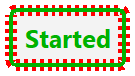
\includegraphics[scale=.2]{figs/maude-testStart}
}\qquad\qquad
\subcaptionbox{Rule \markInputR\label{fig:maude-markInput}}{
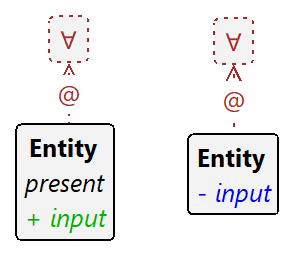
\includegraphics[scale=.2]{figs/maude-markInput}
}
\subcaptionbox{Condition \steadyR\label{fig:maude-steady}}{
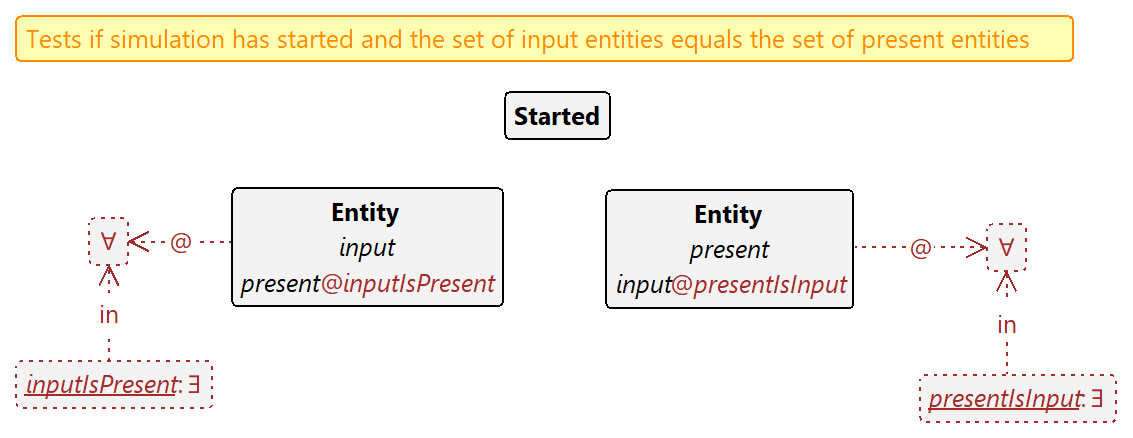
\includegraphics[scale=.2]{figs/maude-steady}
}
\caption{Additional rules and condition for detecting steadiness}
\label{fig:maude-mc}
\end{figure}

\begin{enumerate}
\item Given the context \verb=[k,ket]=, \GROOVE confirms the status of the following LTL properties:
\begin{itemize}
\item \verb=FG(steady -> akt)= is not satisfied; \GROOVE produces a counter-example.

\item \verb=G(erbb2 -> X(erbb2))= is satisfied.
\end{itemize}

\item Given the context \verb=[{e,egf,hrg}.korep]=, \GROOVE confirms the status of the following CTL properties:
\begin{itemize}
\item \verb=EF (steady & !akt)= is satisfied;
\item \verb=AF (steady & !akt)= is not satisfied.
\end{itemize}

\item Given the context \verb=[k,korept]=, \GROOVE confirms the status of the following LTL properties:
\begin{itemize}
\item \verb=G(pdk1 -> FG(steady -> akt))= is satisfied;
\item \verb=erbb1 R !pdk1= is satisfied.
\end{itemize}

\item Given the context \verb=[k,kge]=, \GROOVE confirms the status of the following CTL property:
\begin{itemize}
\item \verb=EG EF (steady -> !akt)= is satisfied. 
\end{itemize}
However, we want to point out that this property does not actually provide any useful guarantees, because the predicate \verb=steady= (both in \cite{DBLP:conf/cmsb/BallisBFO24} and in our encoding explained above) only tests for \emph{single-state} attractors. If the reaction system ends up in a multi-state loop, \verb=steady= will never be satisfied and hence the implication \verb=steady -> !akt= is \emph{always} satisfied, irregardless of whether or not \verb=akt= holds. Indeed, the state space of this scenario, visually reproduced in \Cref{fig:maude-gts}, has such a multi-state attractor (consisting of states \textit{s15} and \textit{s18}); in both of those states the predicate \verb=akt= holds, yet the state space as a whole satisfies the CTL property above.
\end{enumerate}
%
\begin{figure}\centering
\scalebox{.9}{% To use this figure in your LaTeX document
% import the package groove/resources/groove2tikz.sty
%
\begin{tikzpicture}[scale=.7,name prefix=rs-explore-gts-]
\node[start_node, active] (s0) {\ml{\uline{\textit{s0}}}};
\node[state_node] (s4) [right=.7 of s0] {\ml{\uline{\textit{s4}}\\\textit{erbb1}\\\textit{erbb2}\\\textit{erbb3}\\\textit{erk12}\\\textit{plcg}}};
\node[state_node] (s8) [right=.7 of s4] {\ml{\uline{\textit{s8}}\\\textit{akt}\\\textit{erk12}\\\textit{mek12}\\\textit{p70s6k}\\\textit{pdk1}\\\textit{pkca}\\\textit{plcg}}};
\node[state_node] (s11) [right=.7 of s8] {\ml{\uline{\textit{s11}}\\\textit{akt}\\\textit{erbb1}\\\textit{erbb2}\\\textit{erbb3}\\\textit{erk12}\\\textit{mek12}\\\textit{mtor}\\\textit{p70s6k}\\\textit{pdk1}\\\textit{pkca}\\\textit{plcg}}};
\node[state_node] (s15) [right=.7 of s11] {\ml{\uline{\textit{s15}}\\\textit{akt}\\\textit{erk12}\\\textit{mek12}\\\textit{mtor}\\\textit{p70s6k}\\\textit{pdk1}\\\textit{pkca}\\\textit{plcg}}};
\node[state_node] (s18) [right=.7 of s15] {\ml{\uline{\textit{s18}}\\\textit{akt}\\\textit{erbb1}\\\textit{erbb2}\\\textit{erbb3}\\\textit{erk12}\\\textit{mek12}\\\textit{mtor}\\\textit{p70s6k}\\\textit{pdk1}\\\textit{pkca}\\\textit{plcg}}};

\path[trans_edge](s0.east) -- node[lab] {\ml{fire}} (s4) ;
\path[trans_edge](s4.east) -- node[lab] {\ml{fire}} (s8) ;
\path[trans_edge](s8.east) -- node[lab] {\ml{fire}} (s11) ;
\path[trans_edge](s11.east) -- node[lab] {\ml{fire}} (s15) ;
\path[trans_edge](s15.15) -- node[lab] {\ml{fire}} (s18.165) ;
\path[trans_edge](s18.195) -- node[lab] {\ml{fire}} (s15.345) ;
\end{tikzpicture}
}
\caption{GTS for cancer scenario~4}
\label{fig:maude-gts}
\end{figure}
%
In replicating the results from \cite{DBLP:conf/cmsb/BallisBFO24}, we have had to make a few adjustments. The LTL formulas reported in \cite[Page~14]{DBLP:conf/cmsb/BallisBFO24} for scenarios 1 and~3 are actually \emph{not} literally the ones above, but use the predicate \verb=io-state= rather than \verb=isSteady=. We believe that the use of \verb=isSteady= (or, in our case \steadyR) is more informative and probably the intended version.

As a final observation, we note that the numbers of states in all these scenarios is actually quite small. We have already shown the 6-state scenario~4 in \Cref{fig:maude-gts}; the size of the others is given by the following table.
%
\begin{center}
\begin{tabular}{rlr}
\bf Nr. & \bf Context & \bf States \\
\hline\hline
1 & \tt [k,ket] & 4 \\
2 & \tt [{e,egf,hrg}.korep] & 10 \\
3 & \tt [k,korept] & 32 \\
4 & \tt [k,kge] & 6
\end{tabular}
\end{center}

\subparagraph*{Discussion.}

Compared to the prior results in \cite{DBLP:conf/cmsb/BallisBFO24}, the advantages of using \GROOVE lie in the combination of visual inspection and automatic model checking. Not only were we able to confirm the findings of the original paper using exactly the same encoding of reaction system as for the previous case, but the ability to inspect and visualise the state spaces also gives additional insights, such as the observation above that steadiness as formalised there does not actually capture the intended notion of being an attractor.


% !TEX root =  ./main.tex


\subsection{T cell differentiation analysis}\label{sec:datamod2023}

\textcolor{blue}{The paper~\cite{datamod2023-NaCo} (being the full and corrected version of~\cite{datamod2023}, see also Footnote~\ref{correction})} exploits Reaction Systems to analyse T cell differentiation in the immune system, a widely studied biological phenomenon. The starting point for the analysis is a Boolean network model; several of those are available as a \cite{saez2007logical,thakar2010boolean,puniya2018mechanistic}, among which the one in \cite{puniya2018mechanistic} was selected. The model encompasses reactions enabling T cells to manifest various phenotypes in response to environmental stimuli, and describes a realistic regulation system that is involved in many diseases \cite{lafaille1998role,hirahara2016cd4+,meng2016regulatory}.
% it has been investigated under both the viewpoints of causality (effect of environmental conditions) and of reachability (reachable phenotypes). 

The Boolean network model is graphically represented as shown in Fig.~\ref{fig:model-graph}, where the 9 orange nodes represent different environmental stimuli that the T cell can receive; all the other nodes represent so-called \emph{transcription factors} and have an associated Boolean update formula that specifies when they are triggered. 
%The analysis allowed to uncover the genes necessary for the expression of a target transcription factor.
%The analysis of the model allowed to determine which combinations of stimuli lead to each phenotype, and also which proteins inside T cells are involved in each case. 
T cells can manifest four phenotypes, 
%\texttt{Th1}, \texttt{Th2}, \texttt{Th17} and \texttt{iTreg}, 
represented by the four transcription factors \texttt{tbet}, \texttt{gata3}, \texttt{rorgt} and \texttt{foxp3}, respectively.
%The case in which none of the four relevant transcription factors is expressed (i.e., no phenotype is exhibited) is denoted as Th0.
There exists experimental and computational evidence that a T cell can manifest more than one phenotype \cite{luckheeram2012cd4+,puniya2018mechanistic}.

\begin{figure}[t]
	\begin{center}
		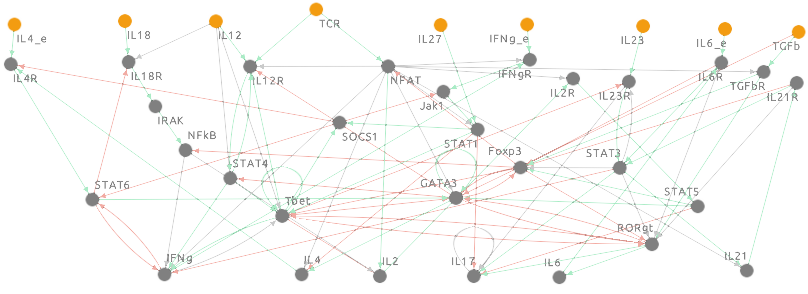
\includegraphics[width=\columnwidth]{figs-datamod2023/Tcell-graph-8set23.png}
	\end{center}
	\caption{Graphical representation of the Boolean network model of T cell differentiation from \cite{puniya2018mechanistic}.}
	\label{fig:model-graph}
\end{figure}

\subparagraph*{Analysis goals.}
The reachability analysis must take into account the different combinations of phenotypes that a T cell can express, called a \emph{target} (hence, $2^4=16$ targets overall).
For example, for the target containing the combination of transcription factors $\{\texttt{tbet},\texttt{gata3}\}$, we must select an attractor that includes at least one state in which $\texttt{tbet}$ is present, at least one state (possibly the same) in which $\texttt{gata3}$ is present, and no state in which either $\texttt{rorgt}$ or $\texttt{foxp3}$ are present. 
The causal analysis aims to collect the combinations of environmental stimuli that are responsible for leading to that target.

\subparagraph*{Features of interest.}
We have selected this case study because it shows the applicability of our method to Boolean networks models, like those available in the public database on the CellCollective platform~\cite{helikar2012cell}. 
For these models, the most relevant viewpoints are often reachability (e.g., \emph{which phenotypes are reachable?}) and causality (\emph{what is the effect of environmental conditions?}) analyses.
Their corresponding RSs always use a special kind of nondeterministic persistent context, where at the beginning of the experiment a subset of external stimuli is chosen and then provided at each subsequent step, inevitably causing the RS to end up in a loop (called an attractor).

\subparagraph*{Experimental set up.}

The translation from Boolean networks to RS consists in turning every update formula into disjunctive normal form. Then, every clause of the disjunction produces a reaction in which (i) reactants are the positive atoms, (ii) inhibitors are the negated atoms and (iii) the updated variable forms a singleton product. 
%
%The RS model of T cell differentiation obtained from the translation of the Boolean model is given in Fig. \ref{fig:RS-reactions}.
%
%\begin{figure}[t]
%\fontsize{7}{0}
%\begin{verbatim}
%react([il4r],[socs1,ifng],[stat6]),         react([tgfb,nfat],[void],[tgfbr]),
%react([tbet],[void],[il12r]),               react([stat4],[gata3],[il2r]),
%react([tcr],[gata3],[il12r]),               react([il12,nfat],[void],[il12r]),
%react([il2r],[void],[stat5]),               react([gata3],[tbet],[gata3]),
%react([stat5],[tgfb,rorgt,foxp3,tbet],[gata3]),
%react([stat6,nfat],[tgfb,rorgt,foxp3,tbet],[gata3]),
%react([stat3],[void],[il23r]),              react([il23,stat3],[tbet],[il23r]), 
%react([tbet],[stat3],[ifng]),               react([nfkb],[void],[ifng]),
%react([stat4,nfkb,nfat],[stat6,stat3],[ifng]),
%react([tgfbr,stat3,il6r],[tbet,gata3,foxp3],[rorgt]),
%react([tgfbr,stat3,il21r],[tbet,gata3,foxp3],[rorgt]),
%react([il21],[void],[il21r]),               react([il18,il12],[stat6],[il18r]),
%react([il6e],[void],[il6r]),                react([il6],[void],[il6r]),
%react([il18r],[void],[irak]),               react([il12r,il12],[gata3],[stat4]),
%react([tbet],[void],[socs1]),               react([stat1],[void],[socs1]),
%react([gata3,nfat],[stat1],[il4]),          react([stat3,nfat],[void],[il21]),
%react([rorgt],[void],[il6]),                react([stat5],[il21r,il6r,gata3],[foxp3]),
%react([stat5],[il21r,stat3,gata3],[foxp3]), react([tgfbr],[il21r,il6r,gata3],[foxp3]),
%react([tgfbr],[il21r,stat3,gata3],[foxp3]), react([tbet],[ifng,il12,rorgt,foxp3],[tbet]),
%react([stat4],[rorgt,foxp3],[tbet]),        react([stat1],[rorgt,foxp3],[tbet]),
%react([il27,nfat],[void],[stat1]),          react([jak1],[void],[stat1]),
%react([il21r],[void],[stat3]),              react([il23r],[void],[stat3]),
%react([il6r],[void],[stat3]),               react([ifngr],[socs1],[jak1]),
%react([il2,nfat],[void],[il2r]),            react([il4e],[void],[il4r]),
%react([il4],[socs1],[il4r]),                react([irak],[foxp3],[nfkb]),
%react([tcr],[foxp3],[nfat]),                react([stat3,il17,il23r],[stat1,stat5],[il17]),
%react([rorgt],[stat1],[il17]),              react([nfat,nfkb],[tbet],[il2]),
%react([ifng,nfat],[void],[ifngr]),          react([ifnge,nfat],[void],[ifngr])
%\end{verbatim}
%\normalsize
%\caption{Reactions of the RS model in BioReSolve syntax.}
%\label{fig:RS-reactions}
%\end{figure}
%
The translation from Boolean network to \BioResolve syntax is done using the directive \verb=main_do(bn2rs)=.
For the readers' convenience, all update formulas and the resulting reactions are reported, respectively, in \Cref{fig:boolean-formulas} and in \Cref{fig:bioresolve:tcell} in the Appendix. 
For example, the update formula for \texttt{IL12R} is
%
\begin{small}
\[
 (\mathtt{IL12} \& \mathtt{NFAT})~|~(\mathtt{STAT4} \& \neg \mathtt{GATA3})~|~ \mathtt{Tbet}~|~(\mathtt{TCR} \& \neg \mathtt{GATA3})
\]
\end{small}
%
which yields the four reactions:\footnote{\label{correction}\textcolor{blue}{The specification analysed in~\cite{datamod2023-NaCo}, on which this paper is based, repairs a minor typo in the original conference version~\cite{datamod2023}. Specifically, the product set of the reaction $\mathtt{({stat4},{gata3},{il12r})}$ was mistakenly written as $\mathtt{il2r}$, omitting the digit $\mathtt{1}$. Unfortunately, since $\mathtt{il2r}$ was also a valid entity, the error was difficult to detect. Though the mistake mildly affected the original results, it turns out that for the analysis reported in this paper there is no difference at all.}}
%
\begin{small}
\[
\begin{array}{c@{{\quad}}c}
\mathtt{(\{il12,nfat\},\emptyset,\{il12r\})}
 & \mathtt{(\{stat4\},\{gata3\},\{il12r\})} \\
\mathtt{(\{tbet\},\emptyset,\{il12r\})}
 & \mathtt{(\{tcr\},\{gata3\},\{il12r\})} \\ 
\end{array} 
\]
\end{small}

The RS context can choose any combination of environmental stimuli that will then persist, i.e., for each possible stimulus $s$ we define the context processes $\mathsf{X}_s \triangleq \{\mathsf{s}\}.\mathsf{X}_s$
%\[
%\begin{array}{rllrll}
%\mathsf{X}_s & \triangleq & \{\mathsf{s}\}.\mathsf{X}'_s + \mathsf{Emp} &\quad
%\mathsf{X}'_s & \triangleq & \{\mathsf{s}\}.\mathsf{X}'_s
%\end{array}
%\]
%
and then take the context $\prod_s (\mathsf{X}_s + \mathsf{Emp})$.
%\[
%\begin{array}{rllrll}
%\mathsf{X1} & \triangleq & \{\mathsf{TGFb}\}.\mathsf{X11} + \mathsf{Emp} &\quad
%\mathsf{X11} & \triangleq & \{\mathsf{TGFb}\}.\mathsf{X11}\\
%\mathsf{X2} & \triangleq & \{\mathsf{IL23}\}.\mathsf{X21} + \mathsf{Emp} &\quad
%\mathsf{X21} & \triangleq & \{\mathsf{IL23}\}.\mathsf{X21}\\
%\mathsf{X3} & \triangleq & \{\mathsf{IL12}\}.\mathsf{X31} + \mathsf{Emp} &\quad
%\mathsf{X31} & \triangleq & \{\mathsf{IL12}\}.\mathsf{X31}\\
%\mathsf{X4} & \triangleq & \{\mathsf{IL18}\}.\mathsf{X41} + \mathsf{Emp} &\quad
%\mathsf{X41} & \triangleq & \{\mathsf{IL18}\}.\mathsf{X41}\\
%\mathsf{X5} & \triangleq & \{\mathsf{IL4e}\}.\mathsf{X51} + \mathsf{Emp} &\quad
%\mathsf{X51} & \triangleq & \{\mathsf{IL4e}\}.\mathsf{X51}\\
%\mathsf{X6} & \triangleq & \{\mathsf{IL27}\}.\mathsf{X61} + \mathsf{Emp} &\quad
%\mathsf{X61} & \triangleq & \{\mathsf{IL27}\}.\mathsf{X61}\\
%\mathsf{X7} & \triangleq & \{\mathsf{IL6e}\}.\mathsf{X71} + \mathsf{Emp} &\quad
%\mathsf{X71} & \triangleq & \{\mathsf{IL6e}\}.\mathsf{X71}\\
%\mathsf{X8} & \triangleq & \{\mathsf{IFNge}\}.\mathsf{X81} + \mathsf{Emp} &\quad
%\mathsf{X81} & \triangleq & \{\mathsf{IFNge}\}.\mathsf{X81}\\
%\mathsf{X9} & \triangleq & \{\mathsf{TCR}\}.\mathsf{X91} + \mathsf{Emp} &\quad
%\mathsf{X91} & \triangleq & \{\mathsf{TCR}\}.\mathsf{X91}\\
%\end{array}
%\]
The resulting LTS has an initial branching into $2^9$ different states, because there are $9$ possible stimuli to be considered. Subsequently, each of the $2^9$ states originates a deterministic computation, leading to some attractors. 

\subparagraph*{Previous approach.}
The paper~\cite{datamod2023-NaCo} presents a toolchain (\BioResolve, SWI-Prolog, Python and Python-to-Prolog binding facilitated by the \verb=swiplserver= Python package) to study the Boolean network model. Roughly, after translating the Boolean network model to RS specifications the whole LTS  is constructed according to any combination of persistent stimuli that can be provided by the context. \BioResolve returns the LTS as a graph in dot format, which is then loaded by a Python script. Then, attractors related with a target of interest are identified by looking for cycles in the LTS, and a slicing algorithm performs some form of causal analysis, to simplify each computation trace by preserving only the relevant causes of those target entities. 
The generation of the LTS is often the bottleneck of the approach, both in terms of time (Prolog performance), but also in terms of space, because \BioResolve can require to allocate a large stack limit size to succeed. 

% 
%Finally, the results of slicing analysis are summarized in Figure \ref{fig:slicing-result}, where it is possibile to see, for each target, which internal genes are \emph{strictly necessary} and which are somehow \emph{relevant} for the expression of the transcription factor of the target. 
%
%Each combination inevitably leads to a looping behaviour (called attractors). Then, the Python script conducts an analysis of the attractors w.r.t. some given \emph{target} entities, and the slicing algorithm performs some form of causal analysis, to simplify each computation trace by preserving only the relevant causes of those  target entities. 

%In Table \ref{tab:context-count} we report the number of different contexts (choices of environmental stimuli) that lead to each target. The table shows only targets that can be reached, and they result to be those in which only one transcription factor is expressed, and those in which Tbet is expressed together with another transcription factor. For each target, the contexts leading to it are summarized in the table by a Boolean formula, while in Figure \ref{fig:input-composition} they are depicted graphically. 
%
%\begin{table}[t]
%	\begin{center}
%		\scriptsize
%		\begin{tabular}{|l|c|l|}
%			\hline
%			{\bf Target} & {\bf Contexts} & {\bf Formula}\\
%			\hline
%			Tbet			&	76 		& (not X11) and (X91) and\\
%			&			& ( ((not X31) and (X61))\\
%			&			& \ \ or ((not X31) and (not X61) and (X71) and (X81))\\
%			&			& \ \ or ((not X31) and (not X51) and (not X61) and (not X71) and (X81))\\
%			&			& \ \ or ((X31) and (X71)) )\\
%			\hline
%			GATA3			&	8		& (not X11) and (not X31) and (X51) and \\
%			&			& (not X61) and (not X81) and (X91) \\
%			\hline
%			Foxp3			&	72		& (not X71) and (not X91) and \\
%			& 			& ( ((X11) and (not X61) and (not X81))\\
%			& 			& \ \ or (X31) )\\
%			\hline
%			RORgt			&	16		& (X11) and (not X31) and (not X61) and (X71) and (X91) \\
%			\hline
%			Tbet,GATA3		&	4		& (not X11) and (not X31) and (X51) and \\ 
%			&			& (not X61) and (not X71) and (X81) and (X91) \\
%			\hline
%			Tbet,Foxp3		&	24		& (X11) and (not X31) and (not X71) and (X91)
%			and 
%			( (X61) or (X81) )  \\
%			\hline
%			Tbet,RORgt		&	48		& (X11) and (X71) and (X91)
%			and ( (X31) or (X61) ) \\
%			\hline
%			%		GATA3,Foxp3		& & \\
%			%		GATA3,Rorgt		& & \\
%			%		Foxp3,Rorgt		& & \\
%			%		Tbet,GATA3,Foxp3	& 0 & $false$\\
%			%		Tbet,GATA3,Rorgt	& & \\
%			%		Tbet,Foxp3,Rorgt	& & \\
%			%		GATA3,Foxp3,Rorgt	& & \\
%			%		Tbet,GATA3,Foxp3,Rorgt	& & \\
%			%		\hline
%			{\bf TOTAL}			& {\bf 248} & \\
%			\hline
%		\end{tabular}
%		\normalsize
%	\end{center}
%	\caption{Summary of contexts leading to each reachable target.}
%	\label{tab:context-count}
%\end{table}
%

%In the end, it is shown that 248 contexts (out of 512) lead to the expression of at least one of the four transcription factors under study, with Tbet, corresponding to phenotype Th1, being expressed in the majority of the cases (152 out of 248), half of the times in combination with another transcription factor.
%% (in 76 cases out of 152). 
%%Also Foxp3 is often expressed (in 96 cases out of 248), while RORgt and GATA3 are less frequent (64 and 12 cases, respectively).
%Moreover, it is observed that:
%\begin{itemize}
%	\item TCR has to be present in order to express any of the phenotypes
%	\item IL23R and IL18R do not contribute to determine any of the phenotypes
%	\item The presence of TGFb mostly discriminates between the expression of either Foxp3/RORgt or tbet/GATA3.
%\end{itemize}


%\begin{figure}[t]
%	\begin{center}
%		\includegraphics[width=12cm]{images/input_composition.png}
%	\end{center}
%	\caption{Graphical representation of the Boolean formula given in Table \ref{tab:context-count} and characterizing contexts leading to each reachable target. Green cells denote that the corresponding environmental stimulus has to be present, red cells denote absences, and white cells denote that the stimulus is irrelevant.}
%	\label{fig:input-composition}
%\end{figure}
%
%
%Fig. \ref{fig:input-composition} allows us to make the following main observations about the role of the environment in the T cell differentiation process:
%\begin{itemize}
%	\item TCR has to be present in order to express any of the phenotypes
%	\item IL23R and IL18R do not contribute to determine any of the phenotypes
%	\item The presence of TGFb mostly discriminates between the expression of either Foxp3/RORgt or tbet/GATA3.
%\end{itemize}
%Moreover, the detailed characterization of the contexts leading to the expression of each phenotype could allow several more specific observations to be done.

%The results of the analysis we conducted partially agree with those of a similar analysis done in \cite{puniya2018mechanistic}. However, there are also some significant differences between the results of the two studies. First of all, in \cite{puniya2018mechanistic} the authors show that it is also possibile to reach configurations in which three or four (i.e., all) phenotypes are expressed. Morevoer, they show that a configuration in which only RORgt is expressed cannot be reached. The Boolean network we started from is exactly the same as the one considered in \cite{puniya2018mechanistic}. The main difference between the two analysis approaches lies in the semantics of the environment: in our case the environment is modelled by a context process that remains the same after the initial non-deterministic choice, while in \cite{puniya2018mechanistic} the analysis is performed by applying a simulation method that allows activity levels and noise to be taken into account for the input species. Hence, the method applied in \cite{puniya2018mechanistic} can lead to a larger range of hypotheses about the modelled system behaviours (such as the possibility for T cell to express more than two phenotypes), while ours is more conservative and consistent with the standard simulation approaches. 

%For each target, slicing analysis is conducted by invoking the \verb=main_do(slice,S)= directive of BioReSolve for each state of each attractor of the target. This is obtained by implementing suitable nested loops in the Python script that, at each iteration, execute BioReSolve through the Python-to-Prolog binding provided by the \verb=swiplserver= package.  
%
%Slicing analysis in BioReSolve requires, in addition to the RS reactions, to provide the specification of a monitor (i.e., a logic formula) to collect the proper information during the model execution (see \cite{BBF2023} for details). Monitored entities are only the transcription factors that the target requires to be present.

%Moreover, the context specification now does not contain the non deterministic choice of the general RS model: it is immediately initialized with a specific configuration of environmental stimuli. Here we show an example of specification of both the context and the monitor for the slicing analysis of one of the states of the target \{ Tbet, RORgt \} reachable when the context does not provide IL12, IL4\_e and INFg\_e (denoted as \verb=x31= \verb=x51= and \verb=x81=, respectively):
%
%\small
%\begin{verbatim}
%mycontext("[x11,x21,x0,x41,x0,x61,x71,x0,x91]").
%mymonitor("[ m0 ]").
%mymondef("[ m0 = ([{il12r,il21,il21r,il23r,il6r,nfat,rorgt,
%                   socs1,stat1,stat3,tbet,tgfbr} inW].no({tbet,rorgt}) 
%                + [-({il12r,il21,il21r,il23r,il6r,nfat,rorgt,
%                  	socs1,stat1,stat3,tbet,tgfbr} inW)].m0) ]").
%\end{verbatim} 
%\normalsize

%We remark that this is a form of causality analysis: for example, one gene that results to be necessary may cause the execution of a chain of reactions leading after some steps to the expression of one of the target transcription factors.
%
%Once necessary and relevant genes for one target are identified, we can look for them in the results of the analysis conducted for the other targets. This leads to a notion of \emph{specificity} that is very important. For example, a gene that is necessary for the expression of a phenotype and that is not relevant for the expression of the other phenotypes (i.e., it is highly specific) is a perfect candidate as a target for a drug aimed at inhibiting the expression of its phenotype.
%
%\begin{figure*}[t]
%	\begin{center}
%		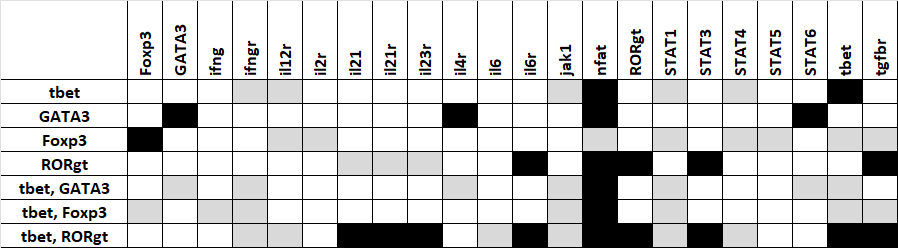
\includegraphics[width=\textwidth]{figs-datamod2023/slicing_results.png}
%	\end{center}
%	\caption{Results of slicing analysis. Black cells identify genes (in columns) that are strictly necessary for the achievement of each target (in rows). Gray cells identify relevant genes. White cells identify genes that are not relevant.}
%	\label{fig:slicing-result}
%\end{figure*}
%
%The table in Figure \ref{fig:slicing-result} allows us to assess necessity, relevance and specificity of each internal gene for each phenotype. In particular, for the four phenotypes characterized by a single transcription factor we can observe that:
%\begin{itemize}
%	\item for target Tbet, the analysis suggests that IFNgR and Jak1 are two relevant genes with high specificity, although they are not strictly necessary for the achievement of the target (i.e., their inhibition or knock-out does not guarantee that the target will not be reached);
%	\item for target GATA3, the analysis suggests that IL4R and STAT6 are strictly necessary and highly specific;
%	\item for target Foxp3, the analysis suggests that IL2R and STAT5 are relevant and highly specific, although not strictly necessary; and
%	\item for target RORgt, the analysis suggests that IL6R and STAT3 are strictly necessary and highly specific, but also IL21, IL21R and IL23 result to be particularly important and specific (as also pointed out in \cite{luckheeram2012cd4+}).
%\end{itemize}
%
%This analysis contributes to the understanding of the behaviour of the model, to correct it in case some mistakes are identified and to use it for identifying drug targets. We discussed the relation with other approaches in the literature.

\subparagraph*{\GROOVE experimentation.}

The capabilities of \GROOVE called upon for this case study are very similar to those in \Cref{sec:cmsb2024}; the main difference lies in the specific interest in attractors. Indeed, in contrast to the situation for comorbidities, here after the initial selection of a profile, the context does not cause any more nondeterminism; hence every profile eventually ends up in such an attractor.

A trace ending in a loop, sometimes called a ``lollipop'', is in fact precisely what LTL properties are checked over; hence an LTL property violation takes the form of a lollipop. This means that we can find attractors with specific properties by formulating their non-existence in LTL, and then generating a counter-example through model checking. For instance, the following formulas deny the reachability of an attractor in which \texttt{tbet} and \texttt{gata3} are expressed:

\begin{itemize}
\item \verb=!G(F gata3 & F tbet)= (separate expression)
\item \verb=!GF (gata3 & tbet)= (simultaneous expression)
\end{itemize}

Using the start graph derived from \BioResolve using the process outlined in \Cref{fig:chain}, both of these formulas yield counterexamples, meaning that \texttt{tbet} and \texttt{gata3} \emph{can} in fact be (recurrently) expressed simultaneously. Using a variation of the process outlined in \Cref{sec:RS2GTS}, we can once more visualise a trace leading to such a recurrent state. The variation lies in the fact that, this time, we do not  want to show the causal history of a \emph{single} forbidden entity, but rather of the combination of two distinct entities. Fortunately, this is just a matter of creating another rule, \gatatbet, which applies precisely when \verb=gata3 & tbet= holds. On this basis we can go through the steps outlined in \Cref{fig:chain}, resulting in the occurrence graph displayed in \Cref{fig:datamod-pruned}.

\begin{figure}\centering
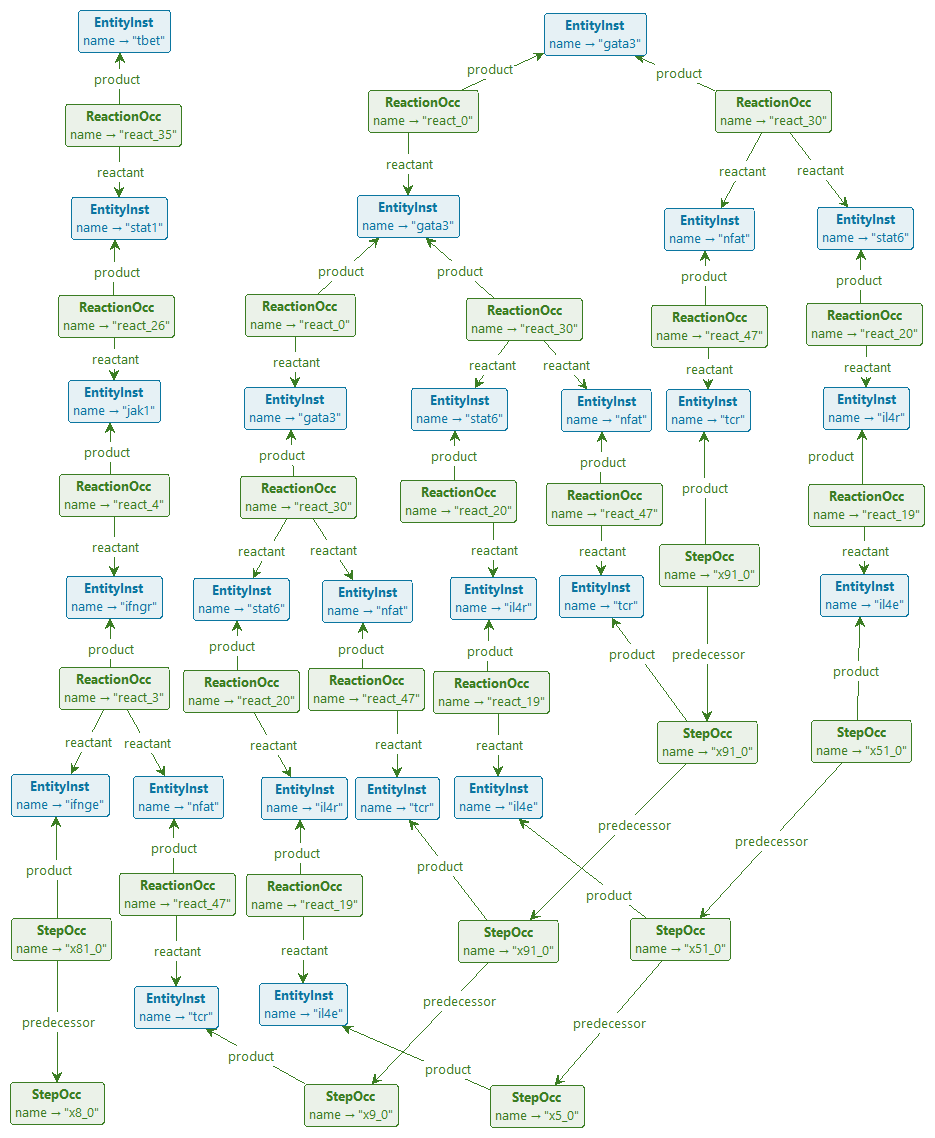
\includegraphics[scale=.25]{figs/datamod-pruned}
\caption{Occurrence graph for the simultaneous expression of \texttt{gata3} and \texttt{tbet}}
\label{fig:datamod-pruned}
\end{figure}

This complements the observation embodied in \cite[Fig.~7]{datamod2023-NaCo} that for the combination of \texttt{tbet} and \texttt{gata3}, the context has to provide the stimuli \texttt{ifnge} (produced here by the \StepOcc named \texttt{x81\_0}), \texttt{tcr} (repeatedly produced by \StepOcc{}s named \texttt{x91\_0}) and \texttt{il4e} (also repeatedly produced, by \StepOcc{}s named \texttt{x51\_0}). In more detail, we see that \texttt{tbet} derives, in a linear sequence of four \ReactionOcc{}s, from \texttt{ifnge} and \texttt{tcr}, whereas \texttt{gata3} derives, in 3 successive combinations of simultaneous \ReactionOcc{}s, from \texttt{tcr} and \texttt{il4e}. Moreover, the genes produced along the way are precisely the ones reported in \cite[Fig.~8(a)]{datamod2023-NaCo}, using the slicing algorithm of that paper, as being relevant for the expression of \texttt{tbet} and \texttt{gata3}.

\medskip\noindent Besides the production of such occurrence graphs for specific cases, \GROOVE can also be used once more to directly confirm the findings of \cite[Figs. 7 and~8]{datamod2023-NaCo}, by expressing them as CTL formulas similar to the one reported in \Cref{fig:table-from-cmsb2024}. In this context, it is relevant to report that, in contrast to \BioResolve, where (as reported above) time and space performance were a bottleneck in the analysis of this model, \GROOVE can fully explore the state space in approximately 3 seconds.

\subparagraph*{Discussion}

Compared to the results in \cite{datamod2023-NaCo}, the advantages of \GROOVE are threefold (reiterating the observations made for the previous two cases):
%
\begin{itemize}
\item LTL model checking allows to express, in a flexible manner, the scenarios one wants to investigate;
\item The occurrence graph visualisation offers analysis possibilities beyond the outcome of the slicing algorithm;
\item The performance of \GROOVE is an order of magnitude better than that of \BioResolve
\end{itemize}




% !TEX root =  ./main.tex

\section{Comparison with Existing Tools}\label{sec:related}

The approach presented in this paper can provide several advantages over existing tools in the literature, including:\footnote{See, e.g., the list of Reaction Systems Computer Environments at \url{https://www.reactionsystems.org/about-reaction-systems}.}
\begin{itemize}
\item
\brsim\footnote{Available at \url{https://github.com/scolobb/brsim/}} (Basic Reaction System Simulator, written in Haskell and distributed under the terms of GNU GPLv3 license)~\cite{DBLP:journals/tcs/AzimiGIP15} was the first RS simulator to be made publicly available. 
Given the reactions of the RS and a context sequence, \brsim is capable of computing the resulting sequence and generating additional annotations for each computation step, such as the enabled reactions.
Alternatively, \brsim can be executed in an interactive mode, allowing the user to manually provide the context to be used at each step.
\item
\WebRSim\footnote{Available at \url{https://github.com/scolobb/brsim}.} is a basic RS simulator that makes all functionalities of  \brsim available through a friendly web interface~\cite{DBLP:conf/birthday/0001RAP18};
\item 
\HERESY\footnote{Available at \url{https://github.com/aresio/HERESY}.} is a Highly Efficient REaction SYstem GPU-based simulator, developed using CUDA~\cite{DBLP:journals/tcs/AzimiGIP15}. It features a user-friendly GUI and is designed to exploit the high degree of parallelism offered by modern GPUs to handle very large-scale RSs simulations.
\item
\clrs\footnote{Available at \url{https://github.com/mnzluca/cl-rs}.} is an optimized Common Lisp simulator for RSs~\cite{DBLP:journals/fuin/FerrettiLMP20} that can exhibit performances comparable with the GPU-based simulator \textsf{HERESY}. This is achieved by discarding all reactions that cannot produce effects and by encoding RS evolution in terms of matrix-vector multiplications and vector additions.
\item 
\BioResolve\footnote{Available at \url{https://www.di.unipi.it/~bruni/LTSRS/}.} is a Prolog interpreter for Reaction System analysis, first proposed in~\cite{DBLP:journals/tcs/BrodoBF21} and later extended in a series of papers to deal with enhanced features, like delays, duration, monitoring, slicing and guarded contexts~\cite{DBLP:journals/nca/BrodoBFGLM23,DBLP:journals/nc/BrodoBF24,DBLP:conf/cmsb/BowlesBBFGM24}. Many capabilities of \BioResolve has been discussed at length in the previous sections.
\item
\ccReact\footnote{Available at \url{https://depot.lipn.univ-paris13.fr/olarte/reaction-systems-maude}.} is an interacting language for Reaction Systems based on Maude 3.2.1~\cite{DBLP:conf/cmsb/BallisBFO24}, whose key features have been illustrated in \Cref{sec:ccReact}.
\end{itemize}

\subparagraph*{Modeling Capabilities.}
The \GROOVE-based method supports a rich and expressive encoding of RSs, including the most recent features such as the handling of \emph{guarded, recursive, and nondeterministic contexts}.
Among the other tools, such features are only supported by \BioResolve, but it relies on a Prolog backend, which limits scalability and requires external scripting for improving the performance of many analyses whenever large state generation and exploration is necessitated. Tools such as \HERESY, \WebRSim, and \clrs provide lightweight RS simulators but are limited to basic semantics, lacking support for more advanced interactions with the context or advanced verification features. \ccReact supports temporal logic model checking (LTL/CTL), but not recursive contexts. Moreover, the encoding of RSs in \ccReact is manual and less suited to visual inspection or dynamic causal analysis.

\subparagraph*{Performance and Scalability}
The ability of \GROOVE to explore large state spaces efficiently is central to our method. Through configurable exploration strategies and a rule-based control mechanism, \GROOVE handles complex RS instances that involve thousands of reachable configurations. Our experiments demonstrate a substantial improvement in analysis time compared to \BioResolve, often reducing execution time by an order of magnitude. Furthermore, the performance of \BioResolve is strongly influenced by the nature of Prolog evaluation strategies, which can lead to excessive memory and time consumption in large case studies.
In contrast, other tools either consider linear executions only and do not scale to large models or lack optimization strategies necessary for handling non-trivial state spaces. 

\subparagraph*{Causal Analysis and Verification.}
A key distinguishing feature of our approach is the ability to perform graph-based \emph{causal slicing}. By automatically generating and pruning \emph{occurrence graphs}, \GROOVE provides detailed and visual explanations of how specific states, such as those involving undesirable or forbidden entities, are reached.
This form of causal reasoning is not available in high-performance tools such as \HERESY, \WebRSim, or \clrs, and is only partially addressed in \ccReact, where the focus is primarily on reachability and temporal properties. 
\todo{Should we say something about the comparison of \GROOVE and \ccReact performances?}
\GROOVE's integrated support for CTL and LTL model checking further extends its applicability to behavioral verification, enabling the specification and validation of complex temporal properties. 

\subparagraph*{Summary.}
In conclusion, the combination of expressive modeling, efficient state space exploration, and integrated causal analysis makes \GROOVE a powerful and versatile full-fledged platform for the study of Reaction Systems. It not only generalizes and extends existing tools, but also opens the door to new forms of analysis that were previously impractical or unsupported.












% !TEX root =  ./main.tex

\section{Conclusion and Future Work}\label{sec:conc}


%\textcolor{red}{
%Flexibility of encoding:
%\begin{itemize}
%\item We can modify our system to other RS variants
%\item Do another (small) case study? Durations?
%\end{itemize}
%}

In this work, we have demonstrated how Reaction Systems can be effectively encoded and analyzed within the \GROOVE framework, so to reuse the expressiveness and efficiency of graph transformation techniques. By exploiting quantified rules, the encoding consists of a direct translation from RS specification to a typed graph, which is made automatic in \BioResolve.
Then, \GROOVE enables both exhaustive state space exploration, the extraction of causal information through occurrence graphs and property-based verification based on model checking.

We have used \GROOVE to revisit several case studies from the literature and our experimental results, although preliminary, are promising: \GROOVE not only supports complex RS features such as guarded, nondeterministic and recursive contexts but also significantly improves performance and flexibility compared to existing RS tools.
Moreover, the use of \GROOVE’s recipes and model-checking capabilities opens the door to sophisticated analyses that were previously impractical.

A number of interesting avenues for future research remain open, among which we mention the possibility to extend the methodology to support quantitative RS variants with durations or weights~\cite{DBLP:journals/nca/BrodoBFGLM23}; investigate alternative notions of causality and their representation in graph-based semantics, like dependencies drawn from inhibitors rather than reactants;~\footnote{In this respect, we could, e.g., exploit the semantic-preserving transformation from RSs to Positive RSs proposed in~\cite{DBLP:journals/sttt/BrodoBFGMMP24}.} apply the \GROOVE toolset to further biological case studies, like those available in the CellCollective public repository~\cite{helikar2012cell}, possibly exploiting an automated pipeline for analysis.

Overall, the results show that graph transformation, and \GROOVE in particular, provide a robust and scalable foundation for the specification, execution, and analysis of Reaction Systems.

\backmatter

\bmhead{Supplementary information}

If your article has accompanying supplementary file/s please state so here. 

\bmhead{Acknowledgements}

\section*{Declarations}

\subsection*{Funding}

Research partially supported 
by \textcolor{red}{Other projects}
by the PRIN PNRR 2022 project \emph{Resource Awareness in Programming} (RAP, P2022HXNSC),
by the University of Pisa PRA project \emph{Formal methods for the healthcare domain based on spatial information} (FM4HD, PRA\_2022\_99),
and by the INdAM GNCS project CUP\_E53C22001930001.

\subsection*{Ethical Approval}
This is not applicable.
 
\subsection*{Competing interests}
The authors have no relevant financial or non-financial interests to disclose.

\subsection*{Availability of data and materials}
Data Availability Statement: No Data associated in the manuscript.

\subsection*{Code availability}

\textcolor{red}{Pointer to git repository?}

\subsection*{Author contribution}

All co-authors contributed equally to this work.

\begin{appendices}

% !TEX root =  ./main.tex

\section{Semantic correspondence}

In this paper, we claim, but do not prove, that the \GROOVE semantics correctly captures the Reaction Systems transitions recalled in \Cref{sec:RS}. A complete formal proof is outside the scope of this paper, which focusses on experimental results; however, in this section we provide a sketch of such a proof.

As described in \Cref{sec:RS2GTS}, each GROOVE state is a graph consisting of a fixed part (which is the same in every state) and a variable part. The fixed part contains an encoding of
\begin{enumerate*}[label=\emph{(\roman*)}]
\item the reaction system $\cal A$ itself, with the entities $S$ given as \Entity-typed nodes, and
\item the automata of the context processes, with individual processes corresponding to \Token-typed nodes and states given as \State-typed nodes.
\end{enumerate*} 
The variable part consisting of \present flags on \Entity nodes and a \current-edge from every \Token to a \State. 
\textcolor{blue}{
As observed in Remark~\ref{rem:shortlts}, any RS process $[\mathsf{M}]$ can be written in the form $[\mathsf{Rs}~|~\mathsf{Ks}~|~D]$ where:
\begin{enumerate*}[label=\emph{(\roman*)}]
\item  $\mathsf{Rs}=\prod_i (R_i,I_i,P_i)$ is the parallel composition of all reactions in the system, and never changes along the computation;
\item $\mathsf{Ks}=\prod_j \mathsf{K}_j$ is the parallel composition of all contexts, and 
\item $D$ is the set of currently present entities. 
\end{enumerate*}
}
%An RS state $[\mathsf{M}]$, on the other hand, consists of
%%
%\begin{enumerate*}[label=\emph{(\roman*)}]
%\item sets $D$ of currently present entities,
%\item fixed reactions $(R,I,P)$, and
%\item regular context processes $\mathsf K$.
%\end{enumerate*}

\textcolor{blue}{
A \GROOVE state $G$ is equivalent to an RS process $[\mathsf{\mathsf{Rs}~|~\mathsf{Ks}~|~D}]$ if:
%
\begin{enumerate*}[label=\emph{(\roman*)}]
\item an entity $\mathsf{e}$ is present in $D$ if and only if its \Entity node is flagged as \present in $G$, and
\item there is a one-to-one correspondence of the available contexts $\mathsf{K}_j$ in the RS process and the $\Token$-nodes in $G$, such that the \current state of that \Token is the start state of the automaton for $\mathsf{K}_j$.
\end{enumerate*}
}
%\begin{enumerate*}[label=\emph{(\roman*)}]
%\item the union of all $D$ in $[\mathsf{M}]$ corresponds precisely to the set of \Entity nodes that are flagged as \present in a $G$, and
%\item there is a one-to-one correspondence of the $\mathsf K$ in $[\mathsf{M}]$ and the $\Token$-nodes in $G$, such that the \current state of that \Token is the start state of the automaton for $\mathsf K$.
%\end{enumerate*}

We claim that this equivalence establishes a bisimulation between the \GROOVE and RS state spaces. (It is not an isomorphism for two reasons:
%
\begin{enumerate*}[label=\emph{(\roman*)}]
\item due to structural equivalence, $\mathsf{[M]}$ may contain multiple, overlapping sets $D$ whereas $G$ merely encodes their union;
\item the RS semantics for $\textsf K$ ``consumes'' the process (rules \textit{(Cxt)}--\textit{(Rec)} in \Cref{fig:guardforRS2nd}) whereas $G$ keeps the automaton intact, merely moving the \current pointer.
\end{enumerate*}
%
To prove this claim, we have to show correspondence of the transitions.

Concretely, to any transition carrying the label $\obs{\obs{D}{R',I',C}}{R,I,P}$, there corresponds a single application of the recipe \fireR, which in turn consists of applications of rules \contextR (see \Cref{fig:context}) followed by \reactR (see \Cref{fig:react}).
%
%Concretely, every $\obs{\obs{D}{R',I',C}}{R,I,P}$-labelled transition corresponds to single application of the recipe \fireR, which in turn consists of applications of rules \contextR (see \Cref{fig:context}) followed by \reactR (see \Cref{fig:react}).
%
\begin{figure}
\centering
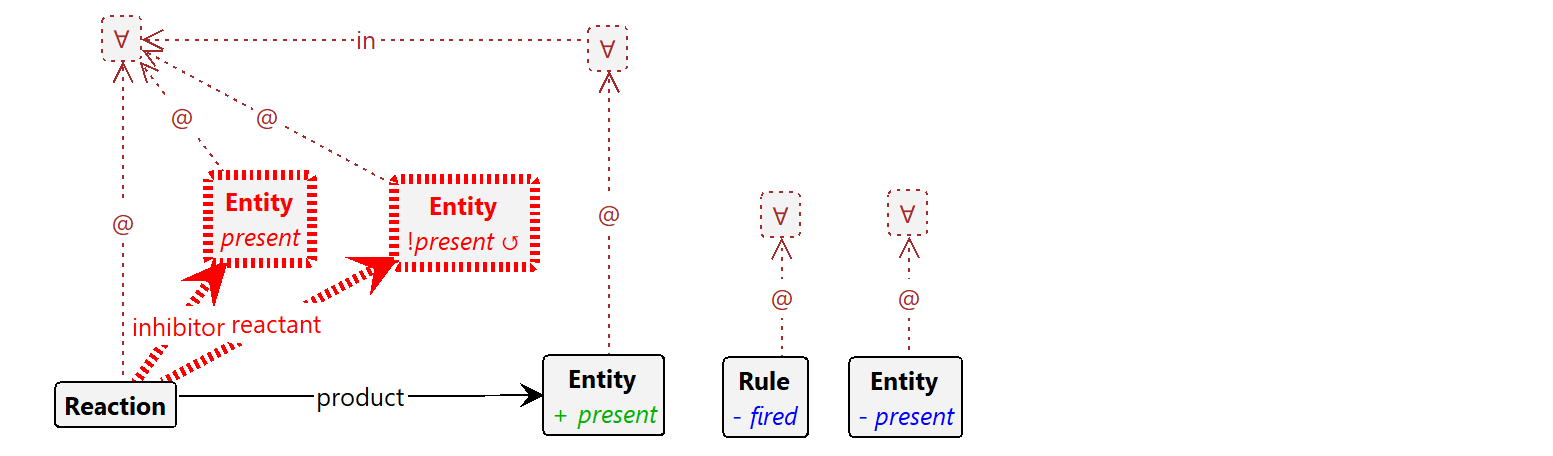
\includegraphics[scale=.2]{figs/react}
\caption{Rule for reaction firing}
\label{fig:react}
\end{figure}
%
Both of these rules are universally quantified. Roughly speaking, referring to \Cref{fig:guardforRS2nd}, \contextR simultaneously encodes all sub-transitions of the form
%
\[\begin{array}{rcll}
D & \xrightarrow{\obs{\obs{D}{\emptyset,\emptyset,\emptyset}}
                     {\emptyset,\emptyset,\emptyset}} & D'
  & \quad\text{\small{(rule (\textit{Ent}))}} \\
\mathsf K
  & \xrightarrow{\obs{\obs{\emptyset}{R',I',C}}
                     {\emptyset,\emptyset,\emptyset}} & \mathsf K'
  & \quad\text{\small{(rules (\textit{Cxt})--(\textit{Rec}))}}
\end{array}\]
%
as well as their composition and filtering (rules (\textit{Par})--(\textit{Sys})). \reactR in turns simultaneously encodes all sub-transitions of the form
%
\[\begin{array}{rcll}
(R,I,P)
  & \xrightarrow{\obs{\obs{\emptyset}
                     {\emptyset,\emptyset,\emptyset}}{R',I',P'}} & \mathsf M'
  & \enspace\text{\small{(rules (\textit{Pro})--(\textit{Inh}))}}
\end{array}\]
%
together with their composition with the \contextR-transitions (rule (\textit{Par})) and filtering (rule (\textit{Sys})). (The \fired-flags on the \Step-nodes, added by \contextR and removed again by \reactR, play no role in this correspondence: for the purpose of the equivalence of the \GROOVE and RS semantics, they might be omitted entirely.)

\section{Auxiliary Material}

\subsection{Auxiliary Material for the toy running example}\label{app:running}

The \BioResolve specification for the toy running example about the interaction between the student and the vending machine is reported in \Cref{fig:bioresolve:toy}. The corresponding RS has been described in \Cref{sec:student} and it has been used to illustrate some key features of the \GROOVE encoding in \Cref{sec:RS2GTS}.

\begin{figure}[t]
\begin{minipage}{0.9\linewidth}
\footnotesize
\begin{verbatim}
myentities([cpowder,tpowder]). % initial set D0

myreactions([                  % list of reactions
    react([idle],[am],[am]),
    react([am],[idle],[am]),
    react([ccoin,cpowder],[nomilk],[cappuccino]),
    react([ccoin,cpowder,nomilk],[],[espresso]),
    react([tcoin,tpowder],[],[tea]),
    react([cpowder],[],[cpowder]),
    react([tpowder],[],[tpowder]),
    react([anger],[],[bang]) ]).

mycontext("[refill,student]"). % context processes

myenvironment("[               % context definitions
    refill = ({nomilk}.refill 
            + {}.refill),
    student = (?{},{am},{tcoin}?.gettea 
             + ?{am},{},{ccoin}?.getcappuccino 
             + {idle}.student),
    gettea = (?{tea},{},{}?.student
            + ?{},{tea},{anger}?.student),
    getcappuccino = (?{cappuccino},{},{}?.student 
                    + ?{espresso},{},{anger}?.student) ]").
\end{verbatim}
\end{minipage}
\caption{\BioResolve implementation of the vending machine RS from \Cref{sec:student}. The question marks \texttt{?} are used to delimit guarded prefixes in context processes.}
\label{fig:bioresolve:toy}
\end{figure}

\subsection{Auxiliary Material for the Comorbidity Case Study}

\newcommand{\ent}[1]{\mathsf{#1}}
\newcommand{\ents}[2]{\mathsf{#1}\texttt{\_}\mathsf{#2}}

The RS specification for the comorbidity case study presented in~\cite{DBLP:conf/cmsb/BowlesBBFGM24} is reported in \Cref{fig:bioresolve:comorbidities:reactions} (set of reactions) and \Cref{fig:bioresolve:comorbidities:contexts} (context processes definitions), where we assume the initial state is $\mathsf{D}_0  =  \varnothing$.
The corresponding experimentation with \GROOVE has been discussed in \Cref{sec:cmsb2024}.

\begin{figure*}[t]
\fontsize{6}{0}
\[
\begin{array}{rcl}
\mathsf{Feats} &  \triangleq 
& (\{\ent{hyper}\},\varnothing,\{\ent{hyper}\})
\mid  (\{\mathsf{afib}\},\varnothing,\{\ent{afib}\})
\mid  (\{\ents{has}{fib}\},\varnothing,\{\ents{has}{fib}\})
\mid  (\{\ents{heart}{rate}\},\varnothing,\{\ents{heart}{rate}\})
\mid  (\{\ents{consensus}{acei}\},\varnothing,\{\ents{consensus}{acei}\})
\\[-4pt] & \mid &  (\{\ent{over75}\},\varnothing,\{\ent{over75}\})
\mid  (\{\ent{below55}\},\varnothing,\{\ent{below55}\})
\mid  (\{\ent{diabete}\},\varnothing,\{\ent{diabete}\})
\mid  (\{\ent{origin}\},\varnothing,\{\ent{origin}\})
\\[-4pt] & \mid &  (\{\ents{doac}{int}\},\varnothing,\{\ents{doac}{int}\})
\mid  (\{\ent{hyper}\},\varnothing,\{\ent{diseases}\})
\mid  (\{\ent{diabete}\},\varnothing,\{\ent{diseases}\})
\\[-4pt]
\mathsf{Drugs} &  \triangleq 
& (\{\ents{get}{diltiazem}\},\{\ents{stop}{cbb}\},\{\ent{diltiazem},\ent{cbb}\})
\mid  (\{\ent{diltiazem}\},\{\ents{stop}{cbb}\},\{\ent{diltiazem},\ent{cbb}\})
\mid  (\{\ents{get}{verapamil}\},\{\ents{stop}{cbb}\},\{\ent{verapamil},\ent{cbb}\})
\\[-4pt] & \mid &  (\{\ent{verapamil}\},\{\ents{stop}{cbb}\},\{\ent{verapamil},\ent{cbb}\})
\mid  (\{\ent{diltiazem},\ent{verapamil}\},\{\ents{stop}{cbb}\},\{\ents{alert}{dup}\})
%
\mid  (\{\ents{get}{propranolol}\},\{\ents{stop}{nsbb}\},\{\ent{propranolol},\ent{nsbb}\})
\\[-4pt] & \mid &  (\{\ent{propranolol}\},\{\ents{stop}{nsbb}\},\{\ent{propranolol},\ent{nsbb}\})
\mid  (\{\ents{get}{carvedilol}\},\{\ents{stop}{nsbb}\},\{\ent{carvedilol},\ent{nsbb}\})
\mid  (\{\ent{carvedilol}\},\{\ents{stop}{nsbb}\},\{\ent{carvedilol},\ent{nsbb}\})
\\[-4pt] & \mid &  (\{\ent{propranolol},\ent{carvedilol}\},\{\ents{stop}{nsbb}\},\{\ents{alert}{dup}\})
%
\mid  (\{\ents{get}{bisoprolol}\},\{\ents{stop}{sbb}\},\{\ent{bisoprolol},\ent{sbb}\})
\mid  (\{\ent{bisoprolol}\},\{\ents{stop}{sbb}\},\{\ent{bisoprolol},\ent{sbb}\})
\\[-4pt] & \mid &  (\{\ents{get}{atenolol}\},\{\ents{stop}{sbb}\},\{\ent{atenolol},\ent{sbb}\})
\mid  (\{\ent{atenolol}\},\{\ents{stop}{sbb}\},\{\ent{atenolol},\ent{sbb}\})
\mid  (\{\ent{bisoprolol},\ent{atenolol}\},\{\ents{stop}{sbb}\},\{\ents{alert}{dup}\})
%
\\[-4pt] & \mid &  (\{\ents{get}{flecainide}\},\{\ents{stop}{flec}\},\{\ent{flecainide}\})
\mid  (\{\ent{flecainide}\},\{\ents{stop}{flec}\},\{\ent{flecainide}\})
\mid  (\{\ents{get}{warfarin}\},\{\ents{stop}{warf}\},\{\ent{warfarin}\})
\\[-4pt] & \mid &  (\{\ent{warfarin}\},\{\ents{stop}{warf}\},\{\ent{warfarin}\})
%
\mid  (\{\ents{get}{apixaban}\},\{\ents{stop}{doac}\},\{\ent{apixaban},\ent{doac}\})
\mid  (\{\ent{apixaban}\},\{\ents{stop}{doac}\},\{\ent{apixaban},\ent{doac}\})
\\[-4pt] & \mid &  (\{\ents{get}{dabigatran}\},\{\ents{stop}{doac}\},\{\ent{dabigatran},\ent{doac}\})
\mid  (\{\ent{dabigatran}\},\{\ents{stop}{doac}\},\{\ent{dabigatran},\ent{doac}\})
\mid  (\{\ent{apixaban},\ent{dabigatran}\},\{\ents{stop}{doac}\},\{\ents{alert}{dup}\})
%
\\[-4pt] & \mid &  (\{\ents{get}{vkant}\},\{\ents{stop}{vkant}\},\{\ent{vkant}\})
\mid  (\{\ent{vkant}\},\{\ents{stop}{vkant}\},\{\ent{vkant}\})
%
\mid  (\{\ents{get}{benazepril}\},\{\ents{stop}{acei}\},\{\ent{benazepril},\ent{acei}\})
\\[-4pt] & \mid &  (\{\ent{benazepril}\},\{\ents{stop}{acei}\},\{\ent{benazepril},\ent{acei}\})
\mid  (\{\ents{get}{captopril}\},\{\ents{stop}{acei}\},\{\ent{captopril},\ent{acei}\})
\mid  (\{\ent{captopril}\},\{\ents{stop}{acei}\},\{\ent{captopril},\ent{acei}\})
\\[-4pt] & \mid &  (\{\ent{benazepril},\ent{captopril}\},\{\ents{stop}{acei}\},\{\ents{alert}{dup}\})
%
\mid  (\{\ents{get}{olmesortan}\},\{\ents{stop}{arb}\},\{\ent{olmesortan},\ent{arb}\})
\mid  (\{\ent{olmesortan}\},\{\ents{stop}{arb}\},\{\ent{olmesortan},\ent{arb}\})
\\[-4pt] & \mid &  (\{\ents{get}{irbesartan}\},\{\ents{stop}{arb}\},\{\ent{irbesartan},\ent{arb}\})
\mid  (\{\ent{irbesartan}\},\{\ents{stop}{arb}\},\{\ent{irbesartan},\ent{arb}\})
\mid  (\{\ent{olmesortan},\ent{irbesartan}\},\{\ents{stop}{arb}\},\{\ents{alert}{dup}\})
%
\\[-4pt] & \mid &  (\{\ents{get}{indapamide}\},\{\ents{stop}{td}\},\{\ent{indapamide},\ent{td}\})
\mid  (\{\ent{indapamide}\},\{\ents{stop}{td}\},\{\ent{indapamide},\ent{td}\})
\mid  (\{\ents{get}{chlorothiazide}\},\{\ents{stop}{td}\},\{\ent{chlorothiazide},\ent{td}\})
\\[-4pt] & \mid &  (\{\ent{chlorothiazide}\},\{\ents{stop}{td}\},\{\ent{chlorothiazide},\ent{td}\})
\mid  (\{\ent{indapamide},\ent{chlorothiazide}\},\{\ents{stop}{td}\},\{\ents{alert}{dup}\})
%
\mid  (\{\ent{doac}\},\{\ents{doac}{ok},\ents{doac}{fail}\},\{\ents{doac}{test}\})
\\[-4pt] & \mid &  (\{\ents{doac}{ok}\},\{\ents{doac}{fail}\},\{\ents{doac}{ok}\})
\mid  (\{\ents{doac}{fail}\},\{\ents{doac}{ok}\},\{\ents{doac}{fail}\})
\mid  (\{\ent{doac}\},\{\ents{doac}{fail},\ents{stop}{doac}\},\{\ents{doac}{danger}\})
\\[-4pt] & \mid &  (\{\ent{doac}\},\{\ents{doac}{danger},\ents{stop}{doac}\},\{\ent{danger}\})
\\[-4pt]
\ent{ADR} &  \triangleq 
& (\{\ents{get}{apixaban},\ents{get}{diltiazem}\},\varnothing,\{\ent{moderate}\})
\mid  (\{\ents{get}{apixaban},\ent{diltiazem}\},\varnothing,\{\ent{moderate}\})
\mid  (\{\ent{apixaban},\ents{get}{diltiazem}\},\varnothing,\{\ent{moderate}\})
\\[-4pt] & \mid &  (\{\ent{apixaban},\ent{diltiazem}\},\varnothing,\{\ent{moderate}\})
\mid  (\{\ents{get}{apixaban},\ents{get}{verapamil}\},\varnothing,\{\ent{moderate}\})
\mid  (\{\ents{get}{apixaban},\ent{verapamil}\},\varnothing,\{\ent{moderate}\})
\\[-4pt] & \mid &  (\{\ent{apixaban},\ents{get}{verapamil}\},\varnothing,\{\ent{moderate}\})
\mid  (\{\ent{apixaban},\ent{verapamil}\},\varnothing,\{\ent{moderate}\})
\mid  (\{\ents{get}{dabigatran},\ents{get}{diltiazem}\},\varnothing,\{\ent{moderate}\})
\\[-4pt] & \mid &  (\{\ents{get}{dabigatran},\ent{diltiazem}\},\varnothing,\{\ent{moderate}\})
\mid  (\{\ent{dabigatran},\ents{get}{diltiazem}\},\varnothing,\{\ent{moderate}\})
\mid  (\{\ent{dabigatran},\ent{diltiazem}\},\varnothing,\{\ent{moderate}\})
\\[-4pt] & \mid &  (\{\ents{get}{dabigatran},\ents{get}{verapamil}\},\varnothing,\{\ent{major}\})
\mid  (\{\ents{get}{dabigatran},\ent{verapamil}\},\varnothing,\{\ent{major}\})
\mid  (\{\ent{dabigatran},\ents{get}{verapamil}\},\varnothing,\{\ent{major}\})
\\[-4pt] & \mid &  (\{\ent{dabigatran},\ent{verapamil}\},\varnothing,\{\ent{major}\})
\mid  (\{\ents{get}{dabigatran},\ents{get}{carvedilol}\},\varnothing,\{\ent{moderate}\})
\mid  (\{\ents{get}{dabigatran},\ent{carvedilol}\},\varnothing,\{\ent{moderate}\})
\\[-4pt] & \mid &  (\{\ent{dabigatran},\ents{get}{carvedilol}\},\varnothing,\{\ent{moderate}\})
\mid  (\{\ent{dabigatran},\ent{carvedilol}\},\varnothing,\{\ent{moderate}\})
\mid  (\{\ents{get}{warfarin},\ents{get}{benazepril}\},\varnothing,\{\ent{minor}\})
\\[-4pt] & \mid &  (\{\ents{get}{warfarin},\ent{benazepril}\},\varnothing,\{\ent{minor}\})
\mid  (\{\ent{warfarin},\ents{get}{benazepril}\},\varnothing,\{\ent{minor}\})
\mid  (\{\ent{warfarin},\ent{benazepril}\},\varnothing,\{\ent{minor}\})
\\[-4pt] & \mid &  (\{\ents{get}{warfarin},\ents{get}{indapamide}\},\varnothing,\{\ent{minor}\})
\mid  (\{\ents{get}{warfarin},\ent{indapamide}\},\varnothing,\{\ent{minor}\})
\mid  (\{\ent{warfarin},\ents{get}{indapamide}\},\varnothing,\{\ent{minor}\})
\\[-4pt] & \mid &  (\{\ent{warfarin},\ent{indapamide}\},\varnothing,\{\ent{minor}\})
\mid  (\{\ents{get}{warfarin},\ents{get}{chlorothiazide}\},\varnothing,\{\ent{minor}\})
\mid  (\{\ents{get}{warfarin},\ent{chlorothiazide}\},\varnothing,\{\ent{minor}\})
\\[-4pt] & \mid &  (\{\ent{warfarin},\ents{get}{chlorothiazide}\},\varnothing,\{\ent{minor}\})
\mid  (\{\ent{warfarin},\ent{chlorothiazide}\},\varnothing,\{\ent{minor}\})
\mid  (\{\ents{get}{warfarin},\ents{get}{propranolol}\},\varnothing,\{\ent{minor}\})
\\[-4pt] & \mid &  (\{\ents{get}{warfarin},\ent{propranolol}\},\varnothing,\{\ent{minor}\})
\mid  (\{\ent{warfarin},\ents{get}{propranolol}\},\varnothing,\{\ent{minor}\})
\mid  (\{\ent{warfarin},\ent{propranolol}\},\varnothing,\{\ent{minor}\})
\\[-4pt] & \mid &  (\{\ents{get}{flecainide},\ents{get}{diltiazem}\},\varnothing,\{\ent{major}\})
\mid  (\{\ents{get}{flecainide},\ent{diltiazem}\},\varnothing,\{\ent{major}\})
\mid  (\{\ent{flecainide},\ents{get}{diltiazem}\},\varnothing,\{\ent{major}\})
\\[-4pt] & \mid &  (\{\ent{flecainide},\ent{diltiazem}\},\varnothing,\{\ent{major}\})
\mid  (\{\ents{get}{flecainide},\ents{get}{verapamil}\},\varnothing,\{\ent{major}\})
\mid  (\{\ents{get}{flecainide},\ent{verapamil}\},\varnothing,\{\ent{major}\})
\\[-4pt] & \mid &  (\{\ent{flecainide},\ents{get}{verapamil}\},\varnothing,\{\ent{major}\})
\mid  (\{\ent{flecainide},\ent{verapamil}\},\varnothing,\{\ent{major}\})
\mid  (\{\ents{get}{flecainide},\ents{get}{bisoprolol}\},\varnothing,\{\ent{moderate}\})
\\[-4pt] & \mid &  (\{\ents{get}{flecainide},\ent{bisoprolol}\},\varnothing,\{\ent{moderate}\})
\mid  (\{\ent{flecainide},\ents{get}{bisoprolol}\},\varnothing,\{\ent{moderate}\})
\mid  (\{\ent{flecainide},\ent{bisoprolol}\},\varnothing,\{\ent{moderate}\})
\\[-4pt] & \mid &  (\{\ents{get}{flecainide},\ents{get}{atenolol}\},\varnothing,\{\ent{moderate}\})
\mid  (\{\ents{get}{flecainide},\ent{atenolol}\},\varnothing,\{\ent{moderate}\})
\mid  (\{\ent{flecainide},\ents{get}{atenolol}\},\varnothing,\{\ent{moderate}\})
\\[-4pt] & \mid &  (\{\ent{flecainide},\ent{atenolol}\},\varnothing,\{\ent{moderate}\})
\mid  (\{\ents{get}{flecainide},\ents{get}{propranolol}\},\varnothing,\{\ent{moderate}\})
\mid  (\{\ents{get}{flecainide},\ent{propranolol}\},\varnothing,\{\ent{moderate}\})
\\[-4pt] & \mid &  (\{\ent{flecainide},\ents{get}{propranolol}\},\varnothing,\{\ent{moderate}\})
\mid  (\{\ent{flecainide},\ent{propranolol}\},\varnothing,\{\ent{moderate}\})
\mid  (\{\ents{get}{flecainide},\ents{get}{carvedilol}\},\varnothing,\{\ent{moderate}\})
\\[-4pt] & \mid &  (\{\ents{get}{flecainide},\ent{carvedilol}\},\varnothing,\{\ent{moderate}\})
\mid  (\{\ent{flecainide},\ents{get}{carvedilol}\},\varnothing,\{\ent{moderate}\})
\mid  (\{\ent{flecainide},\ent{carvedilol}\},\varnothing,\{\ent{moderate}\})
\\[-4pt] & \mid &  (\{\ent{major}\},\varnothing,\{\ent{major}\})
\mid  (\{\ent{moderate}\},\varnothing,\{\ent{moderate}\})
\mid  (\{\ent{minor}\},\varnothing,\{\ent{minor}\})
\mid  (\{\ents{alert}{dup}\},\varnothing,\{\ents{alert}{dup}\})
\mid  (\{\ent{danger}\},\varnothing,\{\ent{danger}\})
\end{array}
\]
\normalsize
\caption{Reactions for the comorbidity case study in~\Cref{sec:cmsb2024}.}
\label{fig:bioresolve:comorbidities:reactions}
\end{figure*}

\begin{figure*}[t]
\fontsize{6}{0}
\[
\begin{array}{rcl}
\ent{eafib1} &  \triangleq 
& (\varnothing,\{\ent{afib}\},\varnothing).\ent{eafib1} 
+ (\{\ent{afib}\},\varnothing,\varnothing).\ent{ehr}
\\[-4pt]
\ent{ehr} &  \triangleq 
& (\varnothing,\{\ents{heart}{rate}\},\varnothing).\ent{ehr} 
+ (\{\ents{heart}{rate}\},\varnothing,\varnothing).\ent{ebb}
\\[-4pt]
\ent{ebb} &  \triangleq 
& \varnothing.\ent{ebb} + \ents{e}{cbb} + \ents{e}{nsbb} + \ents{e}{sbb}
\\[-4pt]
\ents{e}{cbb} &  \triangleq 
& (\varnothing,\{\ent{verapamil}\},\{\ents{get}{diltiazem}\}).\ent{empty} 
+ (\varnothing,\{\ent{diltiazem}\},\{\ents{get}{verapamil}\}).\ent{empty}
\\[-4pt]
\ents{e}{nsbb} &  \triangleq 
& (\varnothing,\{\ent{carvedilol}\},\{\ents{get}{propranolol}\}).\ent{empty} 
+ (\varnothing,\{\ent{propranolol}\},\{\ents{get}{carvedilol}\}).\ent{empty}
\\[-4pt]
\ents{e}{sbb} &  \triangleq 
& (\varnothing,\{\ent{atenolol}\},\{\ents{get}{bisoprolol}\}).\ent{empty} 
+ (\varnothing,\{\ent{bisoprolol}\},\{\ents{get}{atenolol}\}).\ent{empty}
\\[-4pt]
\ent{eafib2} &  \triangleq 
& (\varnothing,\{\ent{afib}\},\varnothing).\ent{eafib2} 
+ (\{\ent{afib}\},\varnothing,\varnothing).\ent{ehf}
\\[-4pt]
\ent{ehf} &  \triangleq 
& (\varnothing,\{\ents{has}{fib}\},\varnothing).\ent{ehf} 
+ (\{\ents{has}{fib}\},\varnothing,\varnothing).\ent{eflec}
\\[-4pt]
\ent{eflec} &  \triangleq 
& \varnothing.\ent{eflec} + \ents{e}{flec}
\\[-4pt]
\ents{e}{flec} &  \triangleq 
& \{\ents{get}{flecainide}\}.\ent{empty}
\\[-4pt]
\ent{eafib3} &  \triangleq 
& (\varnothing,\{\ent{afib}\},\varnothing).\ent{eafib3} 
+ (\{\ent{afib}\},\varnothing,\varnothing).\ent{econs}
\\[-4pt]
\ent{econs} &  \triangleq 
& (\varnothing,\{\ents{heart}\ent{rate},\ents{has}{fib}\},\varnothing).\ent{econs} 
+ (\varnothing,\{\ents{consensus}{acei}\},\varnothing).\ent{econs} 
+ (\{\ents{consensus}{acei},\ents{heart}{rate}\},\varnothing,\varnothing).\ent{estroke} 
+ (\{\ents{consensus}{acei},\ents{has}{fib}\},\varnothing,\varnothing).\ent{estroke} 
\\[-4pt]
\ent{estroke} &  \triangleq 
& (\varnothing,\{\ent{diseases},\ent{over75}\},\varnothing).\ent{ewarf} 
+ (\{\ent{over75}\},\{\ents{doac}{fail},\ents{doac}{int}\},\varnothing).\ent{edoac} 
+ (\{\ent{diseases}\},\{\ents{doac}{fail},\ents{doac}{int}\},\varnothing).\ent{edoac} 
+ (\{\ent{over75},\ents{doac}{fail}\},\varnothing,\varnothing).\ent{evkant} 
\\[-4pt] 
& + & (\{\ent{over75},\ents{doac}{int}\},\varnothing,\varnothing).\ent{evkant} 
+ (\{\ent{diseases}\},\{\ents{doac}{fail},\varnothing,\varnothing).\ent{evkant} 
+ (\{\ent{diseases}\},\{\ents{doac}{int},\varnothing,\varnothing).\ent{evkant}
\\[-4pt]
\ent{ewarf} &  \triangleq 
& \varnothing.\ent{ewarf} + \ents{e}{warf}
\\[-4pt]
\ents{e}{warf} &  \triangleq 
& \{\ents{get}{warfarin}\}.\ent{empty}
\\[-4pt]
\ent{edoac} &  \triangleq 
& \varnothing.\ent{edoac} + \ents{e}{doac}
\\[-4pt]
\ents{e}{doac} &  \triangleq 
& (\varnothing,\{\ent{dabigatran}\},\{\ents{get}{apixaban}\}).\ents{e}{doacfail} 
+ (\varnothing,\{\ent{apixaban}\},\{\ents{get}{dabigatran}\}).\ents{e}{doacfail}
\\[-4pt]
\ents{e}{doacfail} &  \triangleq 
& (\{\ents{doac}{fail}\},\varnothing,\{\ents{stop}{doac}\}).\ent{evkant} 
+ (\varnothing,\{\ents{doac}{fail}\},\varnothing).\ents{e}{doacfail}
\\[-4pt]
\ent{evkant} &  \triangleq 
& \varnothing.\ent{evkant} + \ents{e}{vkant}
\\[-4pt]
\ents{e}{vkant} &  \triangleq 
& \{\ents{get}{vkant}\}.\ent{empty}
\\[-4pt]
\ent{ghyper} &  \triangleq 
& (\varnothing,\{\ent{hyper}\},\varnothing).\ent{ghyper} 
+ (\{\ent{hyper}\},\varnothing,\varnothing).\ent{g1}
\\[-4pt]
\ent{g1} &  \triangleq 
& (\{\ent{diabete}\},\varnothing,\varnothing).\ent{g2} 
+ (\{\ent{below55}\},\{\ent{diabete},\ent{origin}\},\varnothing).\ent{g2} 
+ (\varnothing,\{\ent{below55},\ent{diabete}\},\varnothing).\ent{g3} 
+ (\{\ent{origin}\},\{\ent{diabete}\},\varnothing).\ent{g3}
\\[-4pt]
\ent{g2} &  \triangleq 
& \varnothing.\ent{g2} 
+ (\varnothing,\{\ent{captopril}\},\{\ents{get}{benazepril}\}).\ent{g4}
+ (\varnothing,\{\ent{benazepril}\},\{\ents{get}{captopril}\}).\ent{g4}
+ (\varnothing,\{\ent{irbesartan}\},\{\ents{get}{olmesortan}\}).\ent{g5}
\\[-4pt]
& + & (\varnothing,\{\ent{olmesortan}\},\{\ents{get}{irbesartan}\}).\ent{g5}
\\[-4pt]
\ent{g3} &  \triangleq 
& \varnothing.\ent{g3} 
+ (\varnothing,\{\ent{verapamil}\},\{\ents{get}{diltiazem}\}).\ent{g6}
+ (\varnothing,\{\ent{diltiazem}\},\{\ents{get}{verapamil}\}).\ent{g6}
\\[-4pt]
\ent{g4} &  \triangleq 
& \varnothing.\ent{g4} 
+ (\varnothing,\{\ent{verapamil}\},\{\ents{get}{diltiazem}\}).\ent{g7}
+ (\varnothing,\{\ent{diltiazem}\},\{\ents{get}{verapamil}\}).\ent{g7}
+ (\varnothing,\{\ent{chlorothiazide}\},\{\ents{get}{indapamide}\}).\ent{g8}
\\[-4pt]
& + & (\varnothing,\{\ent{indapamide}\},\{\ents{get}{chlorothiazide}\}).\ent{g8}
\\[-4pt]
\ent{g5} &  \triangleq 
& \varnothing.\ent{g5} 
+ (\varnothing,\{\ent{verapamil}\},\{\ents{get}{diltiazem}\}).\ent{g9}
+ (\varnothing,\{\ent{diltiazem}\},\{\ents{get}{verapamil}\}).\ent{g9}
+ (\varnothing,\{\ent{chlorothiazide}\},\{\ents{get}{indapamide}\}).\ent{g10}
\\[-4pt]
& + & (\varnothing,\{\ent{indapamide}\},\{\ents{get}{chlorothiazide}\}).\ent{g10}
\\[-4pt]
\ent{g6} &  \triangleq 
& \varnothing.\ent{g6} 
+ (\varnothing,\{\ent{captopril}\},\{\ents{get}{benazepril}\}).\ent{g7}
+ (\varnothing,\{\ent{benazepril}\},\{\ents{get}{captopril}\}).\ent{g7}
+ (\varnothing,\{\ent{irbesartan}\},\{\ents{get}{olmesortan}\}).\ent{g9}
\\[-4pt]
& + & (\varnothing,\{\ent{olmesortan}\},\{\ents{get}{irbesartan}\}).\ent{g9}
+ (\varnothing,\{\ent{chlorothiazide}\},\{\ents{get}{indapamide}\}).\ent{g11}
+ (\varnothing,\{\ent{indapamide}\},\{\ents{get}{chlorothiazide}\}).\ent{g11}
\\[-4pt]
\ent{g7} &  \triangleq 
& \varnothing.\ent{g7} 
+ (\varnothing,\{\ent{irbesartan}\},\{\ents{get}{olmesortan}\}).\ent{etd}
+ (\varnothing,\{\ent{olmesortan}\},\{\ents{get}{irbesartan}\}).\ent{etd}
+ (\varnothing,\{\ent{chlorothiazide}\},\{\ents{get}{indapamide}\}).\ent{earb}
\\[-4pt]
& + & (\varnothing,\{\ent{indapamide}\},\{\ents{get}{chlorothiazide}\}).\ent{earb}
\\[-4pt]
\ent{g8} &  \triangleq 
& \varnothing.\ent{g8} 
+ (\varnothing,\{\ent{irbesartan}\},\{\ents{get}{olmesortan}\}).\ent{ecbb}
+ (\varnothing,\{\ent{olmesortan}\},\{\ents{get}{irbesartan}\}).\ent{ecbb}
+ (\varnothing,\{\ent{verapamil}\},\{\ents{get}{diltiazem}\}).\ent{earb}
\\[-4pt]
& + & (\varnothing,\{\ent{diltiazem}\},\{\ents{get}{verapamil}\}).\ent{earb}
\\[-4pt]
\ent{g9} &  \triangleq 
& \varnothing.\ent{g9} 
+ (\varnothing,\{\ent{captopril}\},\{\ents{get}{benazepril}\}).\ent{etd}
+ (\varnothing,\{\ent{benazepril}\},\{\ents{get}{captopril}\}).\ent{etd}
+ (\varnothing,\{\ent{chlorothiazide}\},\{\ents{get}{indapamide}\}).\ent{eacei}
\\[-4pt]
& + & (\varnothing,\{\ent{indapamide}\},\{\ents{get}{chlorothiazide}\}).\ent{eacei}
\\[-4pt]
\ent{g10} &  \triangleq 
& \varnothing.\ent{g10} 
+ (\varnothing,\{\ent{captopril}\},\{\ents{get}{benazepril}\}).\ent{ecbb}
+ (\varnothing,\{\ent{benazepril}\},\{\ents{get}{captopril}\}).\ent{ecbb}
+ (\varnothing,\{\ent{chlorothiazide}\},\{\ents{get}{indapamide}\}).\ent{eacei}
\\[-4pt]
& + & (\varnothing,\{\ent{indapamide}\},\{\ents{get}{chlorothiazide}\}).\ent{eacei}
\\[-4pt]
\ent{g11} &  \triangleq 
& \varnothing.\ent{g11} 
+ (\varnothing,\{\ent{captopril}\},\{\ents{get}{benazepril}\}).\ent{earb}
+ (\varnothing,\{\ent{benazepril}\},\{\ents{get}{captopril}\}).\ent{earb}
+ (\varnothing,\{\ent{irbesartan}\},\{\ents{get}{olmesortan}\}).\ent{eacei}
\\[-4pt]
& + & (\varnothing,\{\ent{olmesortan}\},\{\ents{get}{irbesartan}\}).\ent{eacei}
\\[-4pt]
\ent{ecbb} &  \triangleq 
& \varnothing.\ent{ecbb} + \ents{e}{cbb}
\\[-4pt]
\ent{eacei} &  \triangleq 
& \varnothing.\ent{eacei} + \ents{e}{acei}
\\[-4pt]
\ents{e}{acei} &  \triangleq 
& (\varnothing,\{\ent{captopril}\},\{\ents{get}{benazepril}\}).\ent{empty} 
+ (\varnothing,\{\ent{benazepril}\},\{\ents{get}{captopril}\}).\ent{empty}
\\[-4pt]
\ent{earb} &  \triangleq 
& \varnothing.\ent{earb} + \ents{e}{arb}
\\[-4pt]
\ents{e}{arb} &  \triangleq 
& (\varnothing,\{\ent{irbesartan}\},\{\ents{get}{olmesortan}\}).\ent{empty} 
+ (\varnothing,\{\ent{olmesortan}\},\{\ents{get}{irbesartan}\}).\ent{empty}
\\[-4pt]
\ent{etd} &  \triangleq 
& \varnothing.\ent{etd} + \ents{e}{td}
\\[-4pt]
\ents{e}{td} &  \triangleq 
& (\varnothing,\{\ent{chlorothiazide}\},\{\ents{get}{indapamide}\}).\ent{empty} 
+ (\varnothing,\{\ent{indapamide}\},\{\ents{get}{chlorothiazide}\}).\ent{empty}
\\[-4pt]
\ents{k}{doac} &  \triangleq 
& (\{\ents{doac}{test}\},\varnothing,\{\ents{doac}{ok}\}).\ent{empty} 
+ (\{\ents{doac}{test}\},\varnothing,\{\ents{doac}{fail}\}).\ent{empty}
+ (\varnothing,\{\ents{doac}{test}\},\varnothing).\ents{k}{doac}
\\[-4pt]
\ent{empty} &  \triangleq 
& \varnothing.\ent{empty}
\\[-4pt]
\ent{kafib} &  \triangleq 
& \{\ent{afib}\}.\ent{empty} + \ent{empty}
\\[-4pt]
\ent{khf} &  \triangleq 
& \{\ents{has}{fib}\}.\ent{empty} + \ent{empty}
\\[-4pt]
\ent{khr} &  \triangleq 
& \{\ents{heart}{rate}\}.\ent{empty} + \ent{empty}
\\[-4pt]
\ent{kcons} &  \triangleq 
& \{\ents{consensus}{acei}\}.\ent{empty} + \ent{empty}
\\[-4pt]
\ent{kage} &  \triangleq 
& \{\ent{over75}\}.\ent{empty} + \{\ent{below55}\}.\ent{empty} + \ent{empty}
\\[-4pt]
\ent{kdiabete} &  \triangleq 
& \{\ent{diabete}\}.\ent{empty} + \ent{empty}
\\[-4pt]
\ent{kdoacint} &  \triangleq 
& \{\ents{doac}{int}\}.\ent{empty} + \ent{empty}
\\[-4pt]
\ent{khyper} &  \triangleq 
& \{\ent{hyper}\}.\ent{empty} + \ent{empty}
\\[-4pt]
\ent{korigin} &  \triangleq 
& \{\ent{origin}\}.\ent{empty} + \ent{empty}
\end{array}
\]
\normalsize
\caption{Context process definitions for the comorbidity case study in~\Cref{sec:cmsb2024}.
The initial context is given by the parallel composition of therapies 
$\ent{eafib1}
\mid \ent{eafib2}
\mid \ent{eafib3}
\mid \ent{ghyper}$ and the parallel composition of features
$\ent{kafib}
\mid \ent{khf}
\mid \ent{khr}
\mid \ent{kcons}
\mid \ent{kage}
\mid \ent{kdiabete}
\mid \ent{kdoacint}
\mid \ent{khyper}
\mid \ent{korigin}
\mid \ents{k}{doac}$.}
\label{fig:bioresolve:comorbidities:contexts}
\end{figure*}
%\begin{verbatim}
%myentities([]).
%
%myreactions([
%  react([hyper],[],[hyper]), react([afib],[],[afib]), react([has_fib],[],[has_fib]), react([heart_rate],[],[heart_rate]),
%  react([consensus_acei],[],[consensus_acei]), react([over75],[],[over75]), react([below55],[],[below55]), react([diabete],[],[diabete]),
%  react([origin],[],[origin]), react([doac_int],[],[doac_int]), react([doac],[doac_ok,doac_fail],[doac_test]), react([doac_ok],[doac_fail],[doac_ok]),
%  react([doac_fail],[doac_ok],[doac_fail]), react([hyper],[],[diseases]), react([diabete],[],[diseases]), react([get_diltiazem],[stop_cbb],[diltiazem,cbb]),
%  react([diltiazem],[stop_cbb],[diltiazem,cbb]), react([get_verapamil],[stop_cbb],[verapamil,cbb]), react([verapamil],[stop_cbb],[verapamil,cbb]),
%  react([diltiazem,verapamil],[stop_cbb],[alert_dup]), react([get_propranolol],[stop_nsbb],[propranolol,nsbb]),
%  react([propranolol],[stop_nsbb],[propranolol,nsbb]), react([get_carvedilol],[stop_nsbb],[carvedilol,nsbb]), react([carvedilol],[stop_nsbb],[carvedilol,nsbb]), 
%  react([propranolol,carvedilol],[stop_nsbb],[alert_dup]), react([get_bisoprolol],[stop_sbb],[bisoprolol,sbb]), react([bisoprolol],[stop_sbb],[bisoprolol,sbb]),
%  react([get_atenolol],[stop_sbb],[atenolol,sbb]), react([atenolol],[stop_sbb],[atenolol,sbb]), react([bisoprolol,atenolol],[stop_sbb],[alert_dup]),
%  react([get_flecainide],[stop_flec],[flecainide]), react([flecainide],[stop_flec],[flecainide]), react([get_warfarin],[stop_warf],[warfarin]),
%  react([warfarin],[stop_warf],[warfarin]), react([get_apixaban],[stop_doac],[apixaban,doac]), react([apixaban],[stop_doac],[apixaban,doac]),
%  react([get_dabigatran],[stop_doac],[dabigatran,doac]), react([dabigatran],[stop_doac],[dabigatran,doac]), react([apixaban,dabigatran],[stop_doac],[alert_dup]),
%  react([get_vkant],[stop_vkant],[vkant]), react([vkant],[stop_vkant],[vkant]), react([get_benazepril],[stop_acei],[benazepril,acei]), 
%  react([benazepril],[stop_acei],[benazepril,acei]), react([get_captopril],[stop_acei],[captopril,acei]), react([captopril],[stop_acei],[captopril,acei]),
%  react([benazepril,captopril],[stop_acei],[alert_dup]), react([get_olmesortan],[stop_arb],[olmesortan,arb]), react([olmesortan],[stop_arb],[olmesortan,arb]), 
%  react([get_irbesartan],[stop_arb],[irbesartan,arb]), react([irbesartan],[stop_arb],[irbesartan,arb]), react([olmesortan,irbesartan],[stop_arb],[alert_dup]),
%  react([get_indapamide],[stop_td],[indapamide,td]), react([indapamide],[stop_td],[indapamide,td]), react([get_chlorothiazide],[stop_td],[chlorothiazide,td]), 
%  react([chlorothiazide],[stop_td],[chlorothiazide,td]), react([indapamide,chlorothiazide],[stop_td],[alert_dup]), react([doac,doac_fail],[stop_doac],[doac_danger]),
%  react([doac,doac_danger],[stop_doac],[danger]), react([get_apixaban,get_diltiazem],[],[moderate]), react([get_apixaban,diltiazem],[],[moderate]),
%  react([apixaban,get_diltiazem],[],[moderate]), react([apixaban,diltiazem],[],[moderate]), react([get_apixaban,get_verapamil],[],[moderate]),
%  react([get_apixaban,verapamil],[],[moderate]), react([apixaban,get_verapamil],[],[moderate]), react([apixaban,verapamil],[],[moderate]),
%  react([get_dabigatran,get_diltiazem],[],[moderate]), react([get_dabigatran,diltiazem],[],[moderate]), react([dabigatran,get_diltiazem],[],[moderate]),
%  react([dabigatran,diltiazem],[],[moderate]), react([get_dabigatran,get_verapamil],[],[major]), react([get_dabigatran,verapamil],[],[major]),
%  react([dabigatran,get_verapamil],[],[major]), react([dabigatran,verapamil],[],[major]), react([get_dabigatran,get_carvedilol],[],[moderate]),
%  react([get_dabigatran,carvedilol],[],[moderate]), react([dabigatran,get_carvedilol],[],[moderate]), react([dabigatran,carvedilol],[],[moderate]), 
%  react([get_warfarin,get_benazepril],[],[minor]), react([get_warfarin,benazepril],[],[minor]), react([warfarin,get_benazepril],[],[minor]),
%  react([warfarin,benazepril],[],[minor]), react([get_warfarin,get_indapamide],[],[minor]), react([get_warfarin,indapamide],[],[minor]),
%  react([warfarin,get_indapamide],[],[minor]), react([warfarin,indapamide],[],[minor]), react([get_warfarin,get_chlorothiazide],[],[minor]),
%  react([get_warfarin,chlorothiazide],[],[minor]), react([warfarin,get_chlorothiazide],[],[minor]), react([warfarin,chlorothiazide],[],[minor]),
%  react([get_warfarin,get_propranolol],[],[minor]), react([get_warfarin,propranolol],[],[minor]), react([warfarin,get_propranolol],[],[minor]),
%  react([warfarin,propranolol],[],[minor]), react([get_flecainide,get_diltiazem],[],[major]), react([get_flecainide,diltiazem],[],[major]),
%  react([flecainide,get_diltiazem],[],[major]), react([flecainide,diltiazem],[],[major]), react([get_flecainide,get_verapamil],[],[major]),
%  react([get_flecainide,verapamil],[],[major]), react([flecainide,get_verapamil],[],[major]), react([flecainide,verapamil],[],[major]), 
%  react([get_flecainide,get_bisoprolol],[],[moderate]), react([get_flecainide,bisoprolol],[],[moderate]), react([flecainide,get_bisoprolol],[],[moderate]),
%  react([flecainide,bisoprolol],[],[moderate]), react([get_flecainide,get_atenolol],[],[moderate]), react([get_flecainide,atenolol],[],[moderate]), 
%  react([flecainide,get_atenolol],[],[moderate]), react([flecainide,atenolol],[],[moderate]), react([get_flecainide,get_propranolol],[],[moderate]),
%  react([get_flecainide,propranolol],[],[moderate]), react([flecainide,get_propranolol],[],[moderate]), react([flecainide,propranolol],[],[moderate]), 
%  react([get_flecainide,get_carvedilol],[],[moderate]), react([get_flecainide,carvedilol],[],[moderate]), react([flecainide,get_carvedilol],[],[moderate]),
%  react([flecainide,carvedilol],[],[moderate]), react([major],[],[major]), react([moderate],[],[moderate]),
%  react([minor],[],[minor]), react([alert_dup],[],[alert_dup]), react([danger],[],[danger]) ]).
%
%mycontext("[eafib1,eafib2,eafib3,ghyper,kafib,khf,khr,kcons,kage,kdiabete,kdoacint,khyper,korigin,k_doac]").
%
%myenvironment("[
%  eafib1 = (?{},{afib},{}?.eafib1 + ?{afib},{},{}?.ehr),
%  ehr = (?{},{heart_rate},{}?.ehr + ?{heart_rate},{},{}?.ebb),
%  ebb = ({}.ebb + e_cbb + e_nsbb + e_sbb),
%  e_cbb = (?{},{verapamil},{get_diltiazem}?.empty + ?{},{diltiazem},{get_verapamil}?.empty),
%  e_nsbb = (?{},{carvedilol},{get_propranolol}?.empty + ?{},{propranolol},{get_carvedilol}?.empty),
%  e_sbb = (?{},{atenolol},{get_bisoprolol}?.empty + ?{},{bisoprolol},{get_atenolol}?.empty),
%  eafib2 = (?{},{afib},{}?.eafib2 + ?{afib},{},{}?.ehf),
%  ehf = (?{},{has_fib},{}?.ehf + ?{has_fib},{},{}?.eflec),
%  eflec = ({}.eflec + e_flec),
%  e_flec = {get_flecainide}.empty,
%  eafib3 = (?{},{afib},{}?.eafib3 + ?{afib},{},{}?.econs),
%  econs = (?{},{heart_rate,has_fib},{}?.econs + ?{},{consensus_acei},{}?.econs 
%           + ?{consensus_acei,heart_rate},{},{}?.estroke + ?{consensus_acei,has_fib},{},{}?.estroke),
%  estroke = (?{},{diseases,over75},{}?.ewarf + ?{over75},{doac_fail,doac_int},{}?.edoac + ?{diseases},{doac_fail,doac_int},{}?.edoac 
%           + ?{over75,doac_fail},{},{}?.evkant + ?{over75,doac_int},{},{}?.evkant + ?{diseases,doac_fail},{},{}?.evkant + ?{diseases,doac_int},{},{}?.evkant),
%  ewarf = ({}.ewarf + e_warf),
%  e_warf = {get_warfarin}.empty,
%  edoac = ({}.edoac + e_doac),
%  e_doac = (?{},{dabigatran},{get_apixaban}?.e_doacfail + ?{},{apixaban},{get_dabigatran}?.e_doacfail),
%  e_doacfail = (?{doac_fail},{},{stop_doac}?.evkant + ?{},{doac_fail},{}?.e_doacfail),
%  evkant = ({}.evkant + e_vkant),
%  e_vkant = {get_vkant}.empty,	
%  ghyper = (?{},{hyper},{}?.ghyper + ?{hyper},{},{}?.g1),
%  g1 = (?{diabete},{},{}?.g2 + ?{below55},{diabete,origin},{}?.g2 + ?{},{below55,diabete},{}?.g3 + ?{origin},{diabete},{}?.g3),
%  g2 = ({}.g2 + <1,e_acei>.g4 + <1,e_arb>.g5),
%  g3 = ({}.g3 + <1,e_cbb>.g6),
%  g4 = ({}.g4 + <1,e_cbb>.g7 + <1,e_td>.g8),
%  g5 = ({}.g5 + <1,e_cbb>.g9 + <1,e_td>.g10),
%  g6 = ({}.g6 + <1,e_acei>.g7 + <1,e_arb>.g9 + <1,e_td>.g11),
%  g7 = ({}.g7 + <1,e_arb>.etd + <1,e_td>.earb),
%  g8 = ({}.g8 + <1,e_arb>.ecbb + <1,e_cbb>.earb),
%  g9 = ({}.g9 + <1,e_acei>.etd + <1,e_td>.eacei),
%  g10 = ({}.g10 + <1,e_acei>.ecbb + <1,e_cbb>.eacei),
%  g11 = ({}.g11 + <1,e_acei>.earb + <1,e_arb>.eacei),
%  ecbb = ({}.ecbb + e_cbb),
%  eacei = ({}.eacei + e_acei),
%  e_acei = (?{},{captopril},{get_benazepril}?.empty + ?{},{benazepril},{get_captopril}?.empty),
%  earb = ({}.earb + e_arb),
%  e_arb = (?{},{irbesartan},{get_olmesortan}?.empty + ?{},{olmesortan},{get_irbesartan}?.empty),
%  etd = ({}.etd + e_td),
%  e_td = (?{},{chlorothiazide},{get_indapamide}?.empty + ?{},{indapamide},{get_chlorothiazide}?.empty),
%  k_doac = (?{doac_test},{},{doac_ok}?.empty + ?{doac_test},{},{doac_fail}?.empty + ?{},{doac_test},{}?.k_doac),
%  empty = {}.empty,
%  kafib = ({afib}.empty + empty),
%  khf = ({has_fib}.empty + empty),
%  khr = ({heart_rate}.empty + empty),
%  kcons = ({consensus_acei}.empty + empty),
%  kage = ({over75}.empty + {below55}.empty + empty),
%  kdiabete = ({diabete}.empty + empty),
%  kdoacint = ({doac_int}.empty + empty),
%  khyper = ({hyper}.empty + empty),
%  korigin = ({origin}.empty + empty) ]").
%\end{verbatim}

\subsection{Auxiliary Material for the Protein Signaling Networks Case Study}\label{app:psn}

The \BioResolve specification for the protein signaling networks case study presented in~\cite{DBLP:conf/cmsb/BallisBFO24} is reported in \Cref{fig:bioresolve:psn}. The corresponding experimentation with \GROOVE has been discussed in \Cref{sec:ccReact}.


\begin{figure}[t]
\begin{minipage}{0.9\linewidth}
\footnotesize
\begin{verbatim}
myentities([]).

myreactions([
    react([akt],[],[akt]),
    react([erbb3],[],[akt]),
    react([mtor],[],[akt]),
    react([pdk1],[],[akt]),
    react([erbb1],[e,p],[erbb1]),
    react([egf],[e,p],[erbb1]),
    react([plcg],[e,p],[erbb1]),
    react([erbb2],[e,t,p],[erbb2]),
    react([egf],[e,t,p],[erbb2]),
    react([erbb3],[e,t,p],[erbb2]),
    react([erbb3],[e,p],[erbb3]),
    react([hrg],[e,p],[erbb3]),
    react([erk12],[],[erk12]),
    react([egf],[],[erk12]),
    react([p],[],[erk12]),
    react([mek12],[],[erk12]),
    react([mek12],[],[mek12]),
    react([erbb1],[],[mek12]),
    react([erbb2],[],[mek12]),
    react([erbb3],[],[mek12]),
    react([mtor],[],[mtor]),
    react([p],[],[mtor]),
    react([akt],[],[mtor]),
    react([p70s6k],[],[p70s6k]),
    react([akt],[],[p70s6k]),
    react([mtor],[],[p70s6k]),
    react([erk12],[],[p70s6k]),
    react([pdk1],[],[pdk1]),
    react([erbb1],[],[pdk1]),
    react([erbb2],[],[pdk1]),
    react([erbb3],[],[pdk1]),
    react([mek12],[],[pdk1]),
    react([pkca],[],[pkca]),
    react([plcg],[],[pkca]),
    react([plcg],[],[plcg]),
    react([egf],[],[plcg]),
    react([erbb1],[],[plcg]),
    react([erbb2],[],[plcg]),
    react([erbb3],[],[plcg]) ]).

myenvironment("[
    k = {egf,hrg}.k,
    ket = {e,t}.ket,
    korep = ({e}.korep + {p}.korep),
    korept = ({e}.korept + {p}.korept + {t}.korept),
    kge = (?{erbb1},{},{e}?.kge 
          + ?{erbb2},{},{e}?.kge 
          + ?{},{erbb1,erbb2},{}?.kge) ]").

\end{verbatim}
\end{minipage}
\caption{\BioResolve implementation of the protein signaling network case study from \Cref{sec:ccReact}.}
\label{fig:bioresolve:psn}
\end{figure}

\subsection{Auxiliary Material for the T Cell Differentiation Case Study}\label{app:maude}

The \BioResolve specification derived from the Boolean network model (available at \cite{ModelCellCollective}, see \Cref{fig:boolean-formulas}) of the T cell differentiation case study from \cite{puniya2018mechanistic}, and exploited in \cite{datamod2023} is reported in \Cref{fig:bioresolve:tcell}. The corresponding experimentation with \GROOVE has been discussed in \Cref{sec:datamod2023}.




\begin{figure}[t]
	\begin{center}
		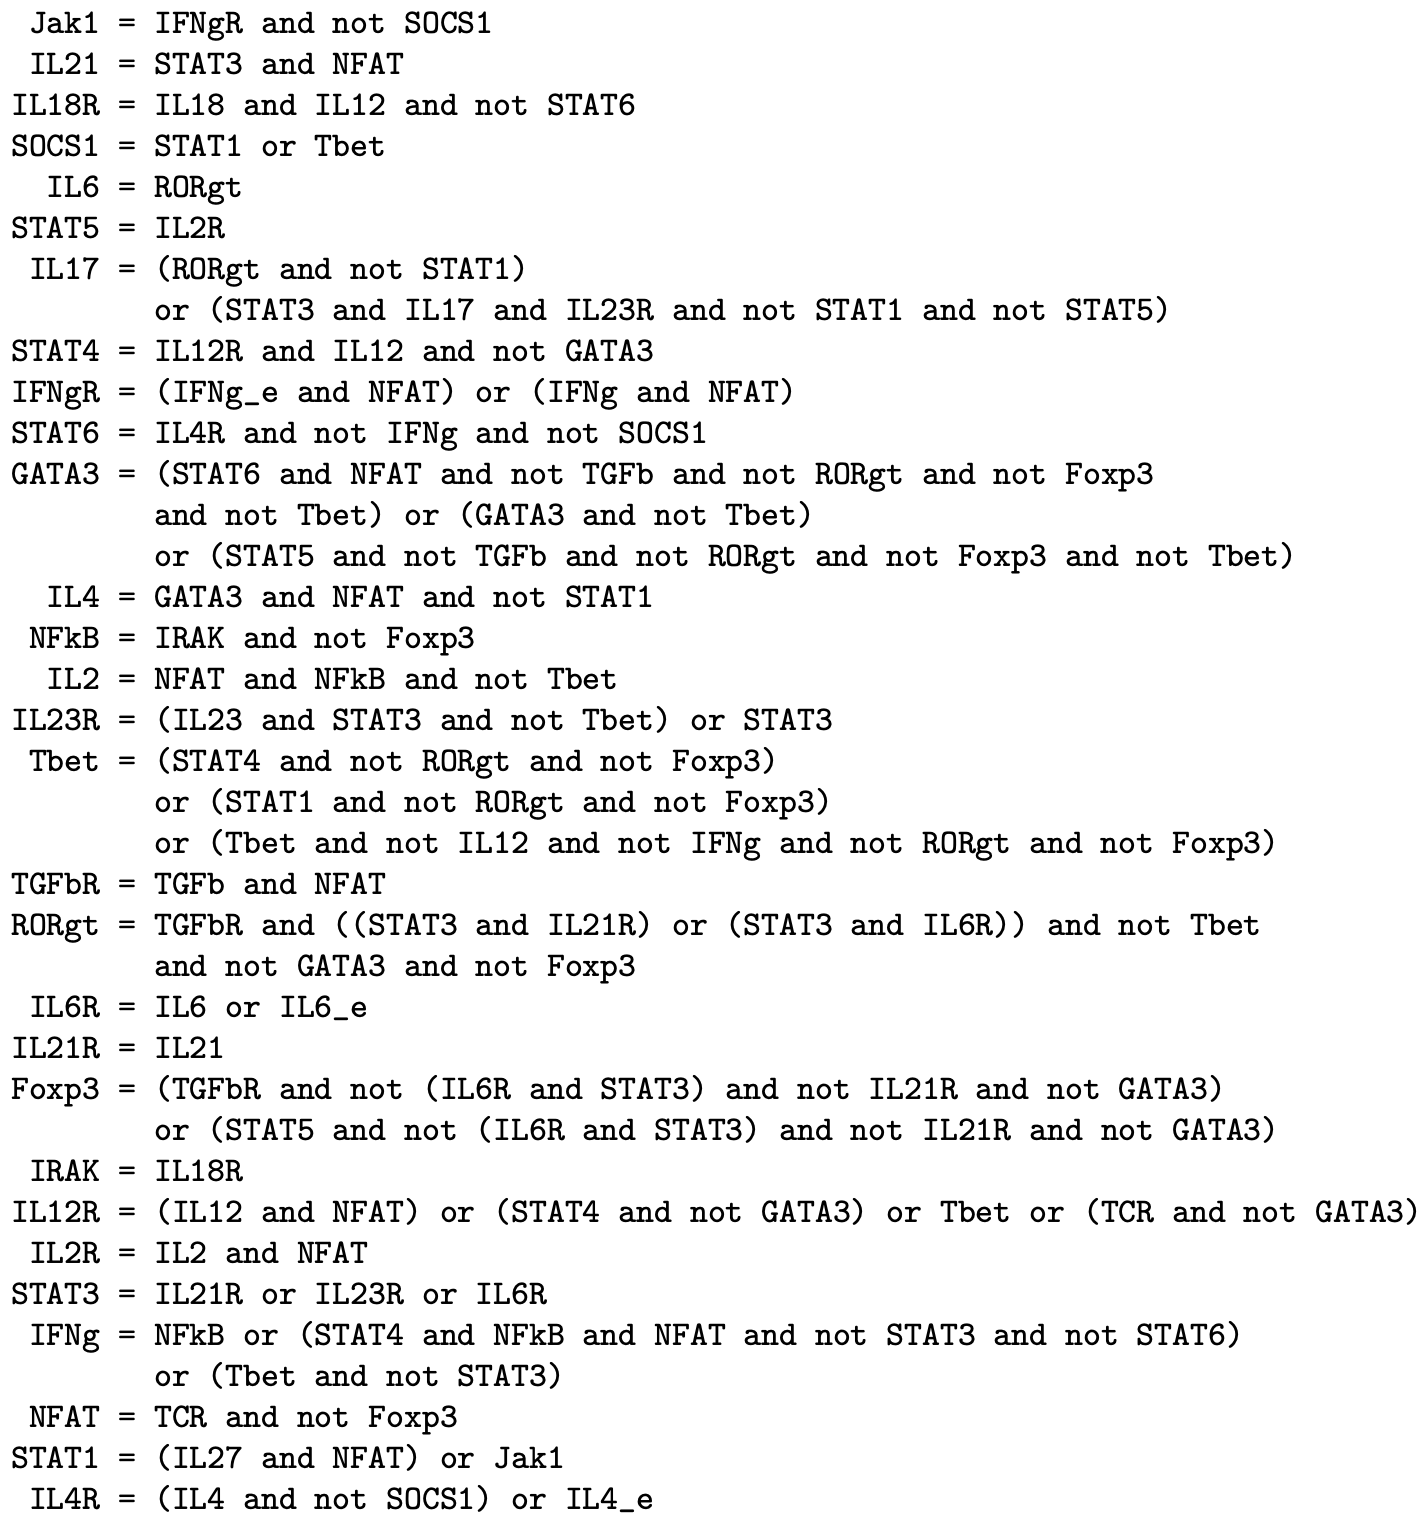
\includegraphics[width=0.49\textwidth]{figs-datamod2023/TcellBN.png}
	\end{center}
%\fontsize{8}{8}
%\begin{verbatim}
% Jak1 = IFNgR and not SOCS1 
% IL21 = STAT3 and NFAT
%IL18R = IL18 and IL12 and not STAT6 
%SOCS1 = STAT1 or Tbet 
%  IL6 = RORgt 
%STAT5 = IL2R 
% IL17 = (RORgt and not STAT1) 
%        or (STAT3 and IL17 and IL23R and not STAT1 and not STAT5) 
%STAT4 = IL12R and IL12 and not GATA3 
%IFNgR = (IFNg_e and NFAT) or (IFNg and NFAT) 
%STAT6 = IL4R and not IFNg and not SOCS1 
%GATA3 = (STAT6 and NFAT and not TGFb and not RORgt and not Foxp3 
%        and not Tbet) or (GATA3 and not Tbet) 
%        or (STAT5 and not TGFb and not RORgt and not Foxp3 and not Tbet) 
%  IL4 = GATA3 and NFAT and not STAT1 
% NFkB = IRAK and not Foxp3 
%  IL2 = NFAT and NFkB and not Tbet 
%IL23R = (IL23 and STAT3 and not Tbet) or STAT3 
% Tbet = (STAT4 and not RORgt and not Foxp3) 
%        or (STAT1 and not RORgt and not Foxp3) 
%        or (Tbet and not IL12 and not IFNg and not RORgt and not Foxp3) 
%TGFbR = TGFb and NFAT 
%RORgt = TGFbR and ((STAT3 and IL21R) or (STAT3 and IL6R)) and not Tbet 
%        and not GATA3 and not Foxp3 
% IL6R = IL6 or IL6_e 
%IL21R = IL21 
%Foxp3 = (TGFbR and not (IL6R and STAT3) and not IL21R and not GATA3) 
%        or (STAT5 and not (IL6R and STAT3) and not IL21R and not GATA3) 
% IRAK = IL18R 
%IL12R = (IL12 and NFAT) or (STAT4 and not GATA3) or Tbet or (TCR and not GATA3) 
% IL2R = IL2 and NFAT 
%STAT3 = IL21R or IL23R or IL6R 
% IFNg = NFkB or (STAT4 and NFkB and NFAT and not STAT3 and not STAT6) 
%        or (Tbet and not STAT3) 
% NFAT = TCR and not Foxp3 
%STAT1 = (IL27 and NFAT) or Jak1 
% IL4R = (IL4 and not SOCS1) or IL4_e 
%\end{verbatim}
	\caption{Boolean updates of the T Cell differentiation model from \cite{puniya2018mechanistic}, available at \cite{ModelCellCollective}.}
	\label{fig:boolean-formulas}
\end{figure}

\begin{figure}[t]
\begin{minipage}{0.9\linewidth}
\footnotesize
\begin{verbatim}
myreactions([
    react([stat5],[gata3,il21r,il6r],[foxp3]),
    react([stat5],[gata3,il21r,stat3],[foxp3]),
    react([tgfbr],[gata3,il21r,il6r],[foxp3]),
    react([tgfbr],[gata3,il21r,stat3],[foxp3]),
    react([gata3],[tbet],[gata3]),
    react([nfat,stat6],[foxp3,rorgt,tbet,tgfb],[gata3]),
    react([stat5],[foxp3,rorgt,tbet,tgfb],[gata3]),
    react([nfat,nfkb,stat4],[stat3,stat6],[ifng]),
    react([nfkb],[],[ifng]),
    react([tbet],[stat3],[ifng]),
    react([ifng,nfat],[],[ifngr]),
    react([ifnge,nfat],[],[ifngr]),
    react([il12,nfat],[],[il12r]),
    react([tbet],[],[il12r]),
    react([tcr],[gata3],[il12r]),
    react([il17,il23r,stat3],[stat1,stat5],[il17]),
    react([rorgt],[stat1],[il17]),
    react([il12,il18],[stat6],[il18r]),
    react([nfat,nfkb],[tbet],[il2]),
    react([nfat,stat3],[],[il21]),
    react([il21],[],[il21r]),
    react([il23,stat3],[tbet],[il23r]),
    react([stat3],[],[il23r]),
    react([il2,nfat],[],[il2r]),
    react([stat4],[gata3],[il2r]),
    react([gata3,nfat],[stat1],[il4]),
    react([il4],[socs1],[il4r]),
    react([il4e],[],[il4r]),
    react([rorgt],[],[il6]),
    react([il6],[],[il6r]),
    react([il6e],[],[il6r]),
    react([il18r],[],[irak]),
    react([ifngr],[socs1],[jak1]),
    react([tcr],[foxp3],[nfat]),
    react([irak],[foxp3],[nfkb]),
    react([il21r,stat3,tgfbr],[foxp3,gata3,tbet],[rorgt]),
    react([il6r,stat3,tgfbr],[foxp3,gata3,tbet],[rorgt]),
    react([stat1],[],[socs1]),
    react([tbet],[],[socs1]),
    react([il27,nfat],[],[stat1]),
    react([jak1],[],[stat1]),
    react([il21r],[],[stat3]),
    react([il23r],[],[stat3]),
    react([il6r],[],[stat3]),
    react([il12,il12r],[gata3],[stat4]),
    react([il2r],[],[stat5]),
    react([il4r],[ifng,socs1],[stat6]),
    react([stat1],[foxp3,rorgt],[tbet]),
    react([stat4],[foxp3,rorgt],[tbet]),
    react([tbet],[foxp3,ifng,il12,rorgt],[tbet]),
    react([nfat,tgfb],[],[tgfbr]) ]).
    
\end{verbatim}
\end{minipage}
\caption{\BioResolve implementation of the T cell case study from \Cref{sec:datamod2023}.}
\label{fig:bioresolve:tcell}
\end{figure}

\subsection{Auxiliary Material for the \GROOVE experiments}\label{app:groove}

To replicate the \GROOVE experiments reported in \Cref{sec:RS2GTS} (for the toy running example) and \Cref{sec:experiments}, we have included the following supplementary resources with this submission:
\begin{itemize}
\item The rule systems described in \Cref{sec:RS2GTS};
\item The start graphs derived from the \BioResolve specifications in this appendix (\ref{app:running}--\ref{app:maude});
\item Instructions for calling the \GROOVE generator so as to reproduce all the exploration runs, occurrence graphs and model checking results (using \href{https://github.com/nl-utwente-groove/code/releases/tag/release-7_4_3}{\GROOVE version 7.4.3}).
\end{itemize}



\end{appendices}


\bibliography{references}



\end{document}
